\documentclass[aspectratio=169]{beamer}
%\documentclass[compact]{beamer}
\usetheme{Hamburg}

\usepackage[T1]{fontenc}
\usepackage[utf8]{inputenc}
\usepackage[english]{babel}
\usepackage{CJKutf8} % for chinese
\usepackage{stmaryrd}
\usepackage{amsmath}
\usepackage{lmodern}

%\usepackage[ngerman]{babel}

\usepackage{eurosym}
\usepackage{listings}
\usepackage{lstautogobble}
\usepackage{microtype}
\usepackage{textcomp}
\usepackage{units}
\DeclareSymbolFont{frenchscript}{OMS}{ztmcm}{m}{n}
%\DeclareMathSymbol{\P}{\mathord}{frenchscript}{65}

% For figures next to each other
\usepackage{graphicx}
\usepackage{graphbox}
\usepackage{subfig}

\usepackage{natbib} % for \citep

\lstset{
	basicstyle=\ttfamily\footnotesize,
	frame=single,
	numbers=left,
	language=C,
	breaklines=true,
	breakatwhitespace=true,
	postbreak=\hbox{$\hookrightarrow$ },
	showstringspaces=false,
	autogobble=true,
	upquote=true,
	tabsize=4,
	captionpos=b,
	morekeywords={int8_t,uint8_t,int16_t,uint16_t,int32_t,uint32_t,int64_t,uint64_t,size_t,ssize_t,off_t,intptr_t,uintptr_t,mode_t}
}

\title[MTACR]{MTACR}

\subtitle{Multilingual Text As Corpus Repository \\Improving Machine Translation of Low-Resource Languages}
\author{Christian Schuler}
\institute{Funded Student's Project\\University of Hamburg and beyond}
\date{\today}

% here you can have a logo, but not necessary
% \titlegraphic{\includegraphics[width=0.15\textwidth]{images/onion.png}}

\begin{document}

\begin{frame}
	\titlepage
\end{frame}

% \begin{frame}
% 	\frametitle{Agenda}
% 	% this hides the subsection
%     % \tableofcontents[hidesubsections]
% 	\tableofcontents
% \end{frame}

\section{Preface}

\begin{frame}[fragile]
	\frametitle{Bachelor's Thesis (2022)}
    \begin{itemize}
        \item Title: Perceptual Quality Assessment of Lip-Synchrony in Dubbing
    \end{itemize}
    \begin{minipage}{.5\textwidth}
      \begin{figure}
        \centering
        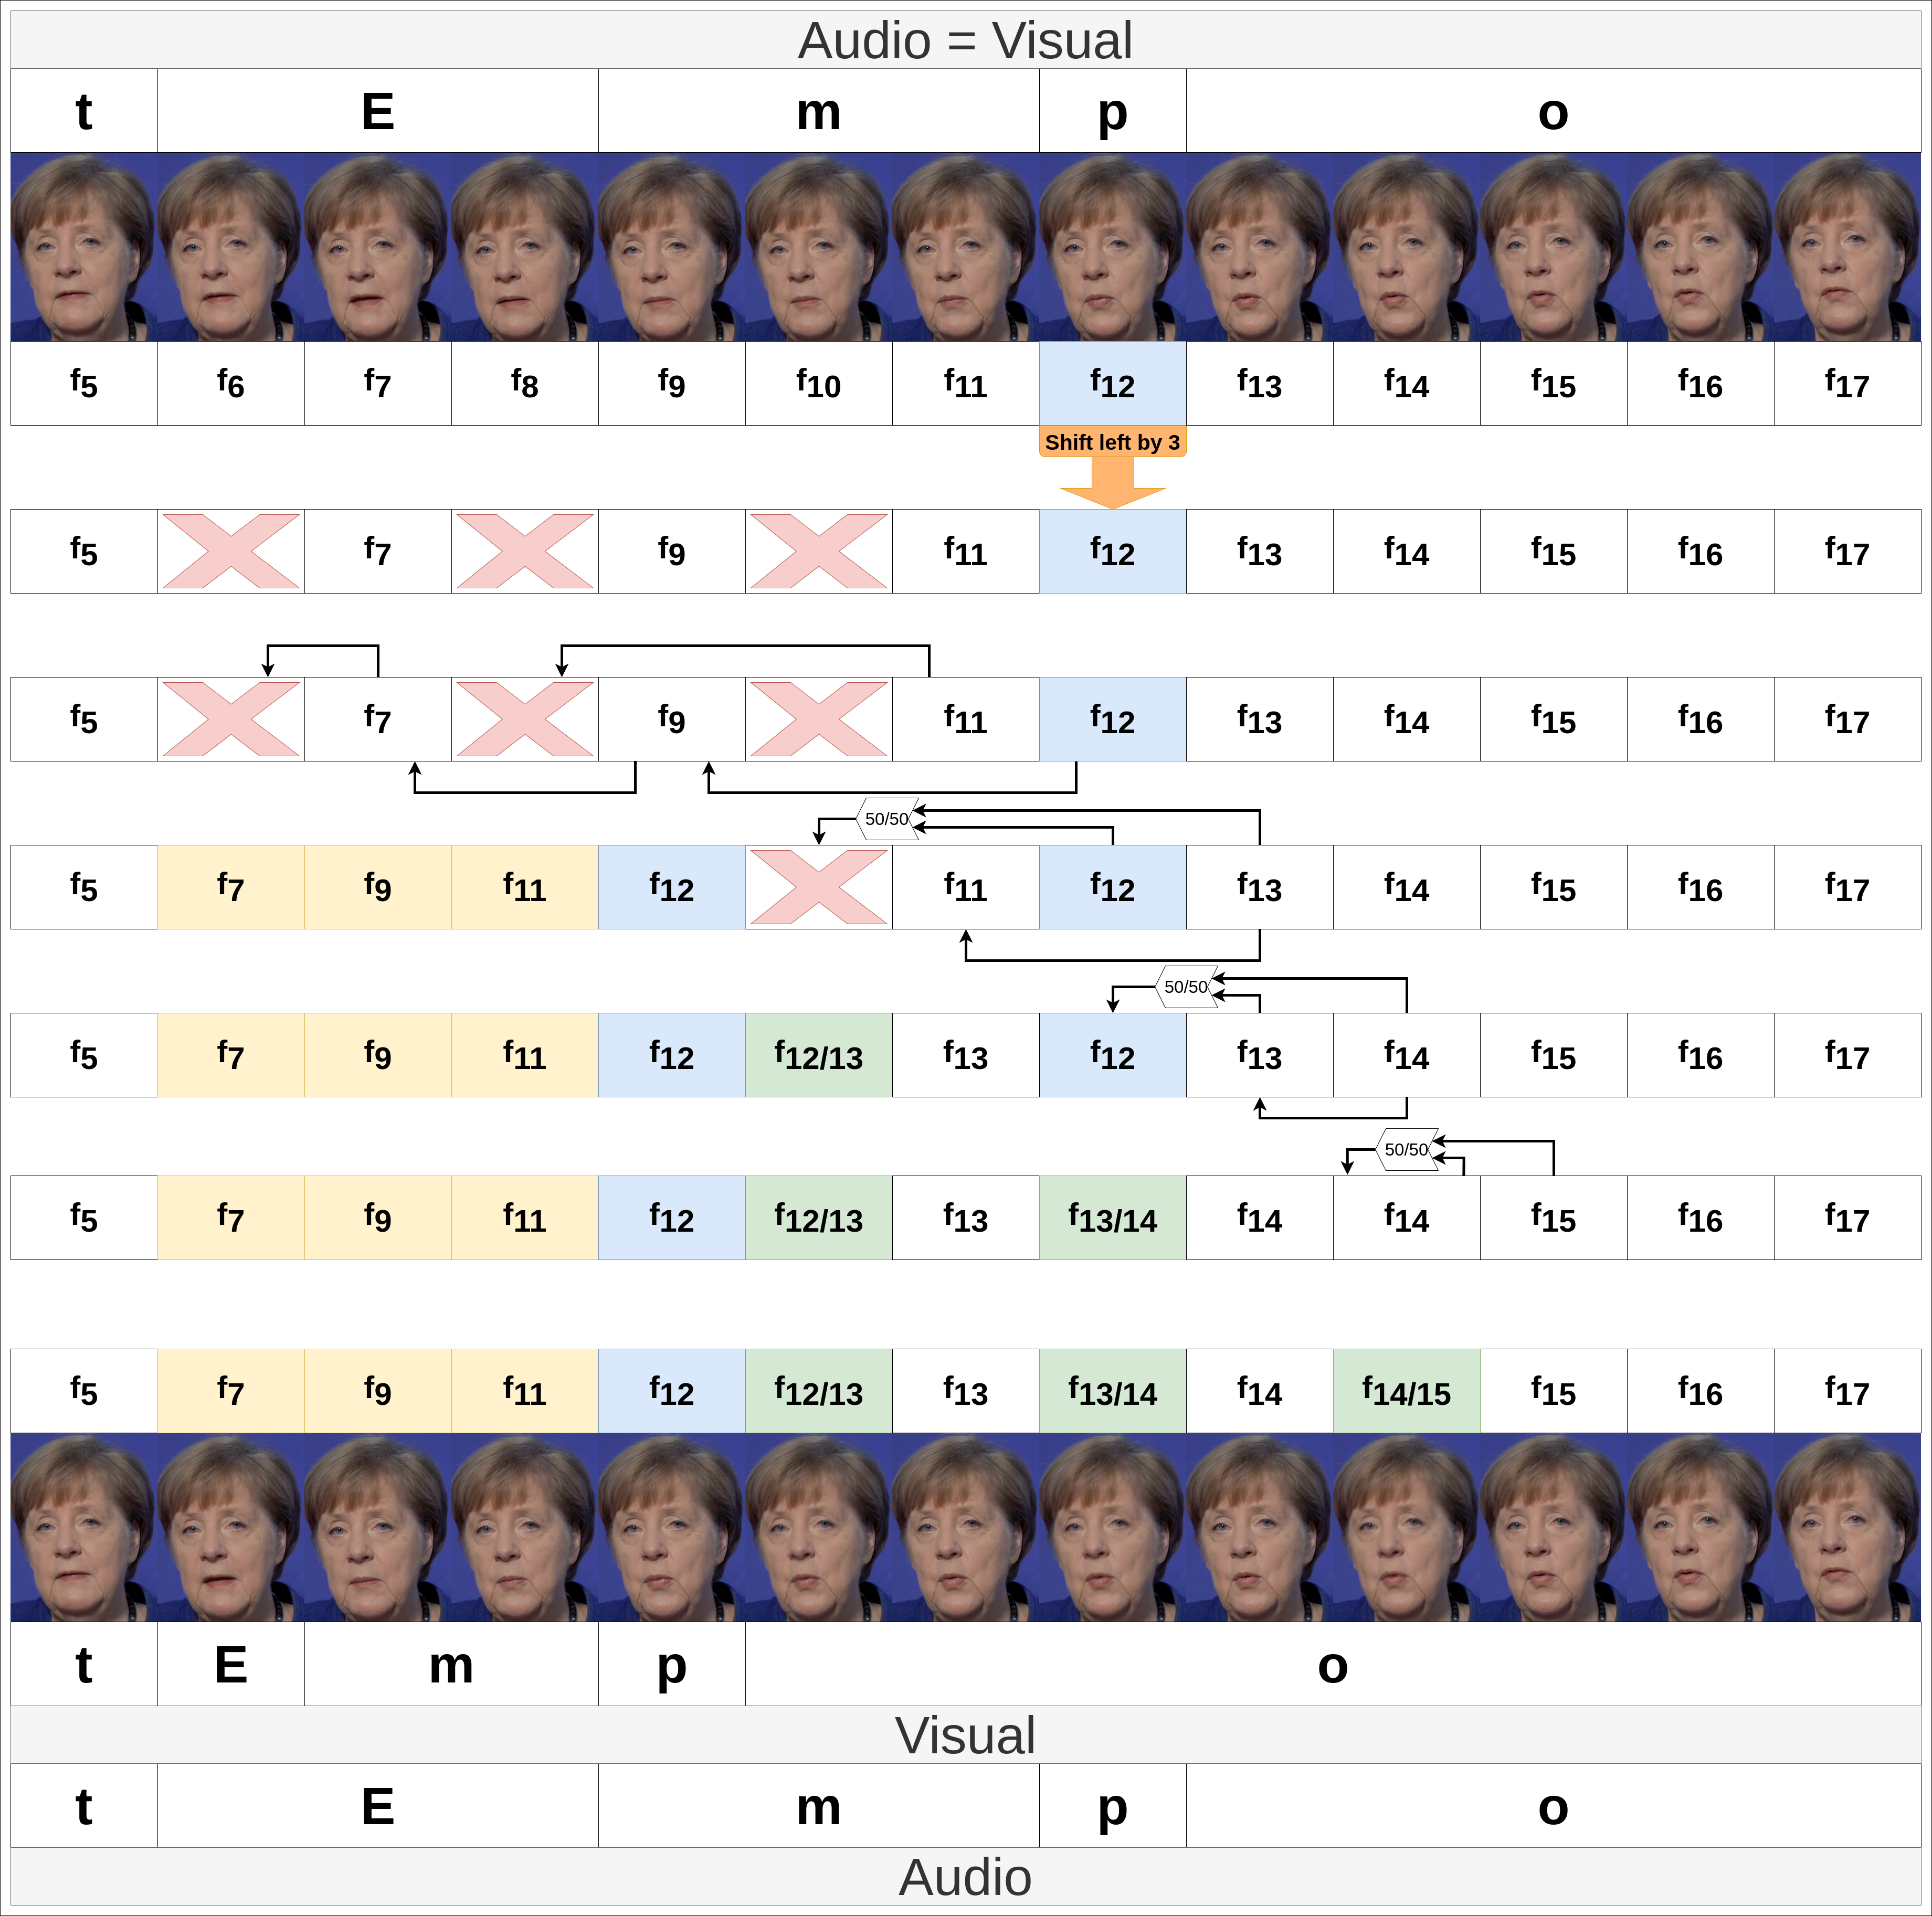
\includegraphics[width=.9\textwidth]{images/DubbingThesisEditing-vL-merkl.png} 
    \end{figure}
    \end{minipage}%
    \begin{minipage}{.5\textwidth}
    \centering
        \begin{minipage}{.3\textwidth}
            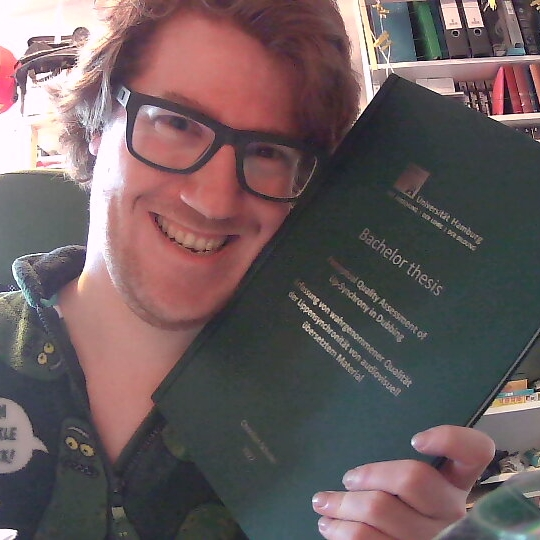
\includegraphics[height=2cm]{images/Christian_Schuler_Thesis.jpg} 
            Christian Schuler
        \end{minipage}
        \begin{minipage}{.3\textwidth}
            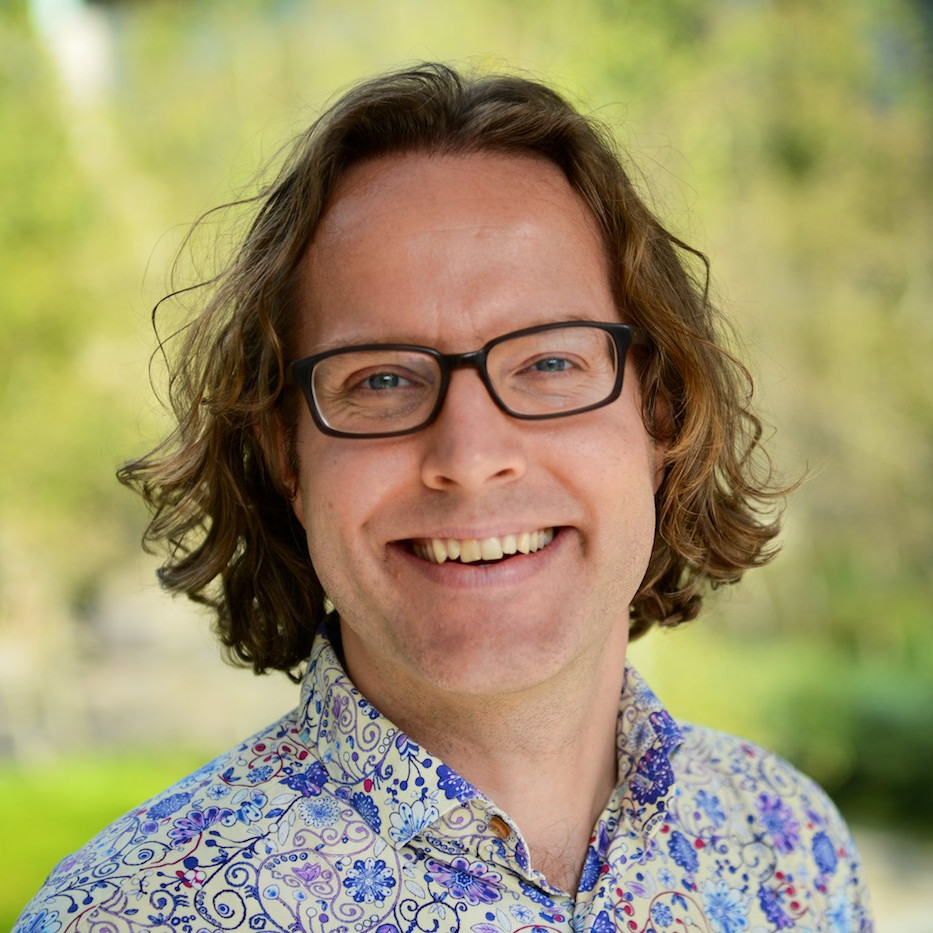
\includegraphics[height=2cm]{images/Timo_Baumann.jpg}
            Dr. Timo\\Baumann
        \end{minipage}
        \begin{minipage}{.3\textwidth}
            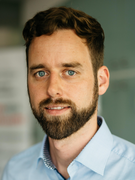
\includegraphics[height=2cm]{images/Timo_Florian_Gerkmann.png}
            Prof. Timo\\Gerkmann
        \end{minipage}
    \end{minipage}
\end{frame}

\begin{frame}[fragile]
	\frametitle{Bachelor's Thesis Fallout (2022-2024)}
    \begin{minipage}{1.0\textwidth}
        \begin{minipage}{.55\textwidth}
            {\color{thiscolor}$\bullet$} Neural synchrony evaluation for audio-visual\\
            translation \citep{nayak2022DeepDiveNeural}
            %A Deep Dive Into Neural Synchrony Evaluation for Audio-visual Translation \citep{nayak2022DeepDiveNeural}
            %\vspace{-8mm}
        \end{minipage}
        \begin{minipage}{.45\textwidth}
            \begin{figure}
            \centering
            \captionsetup[subfigure]{labelformat=empty}
                \subfloat[]{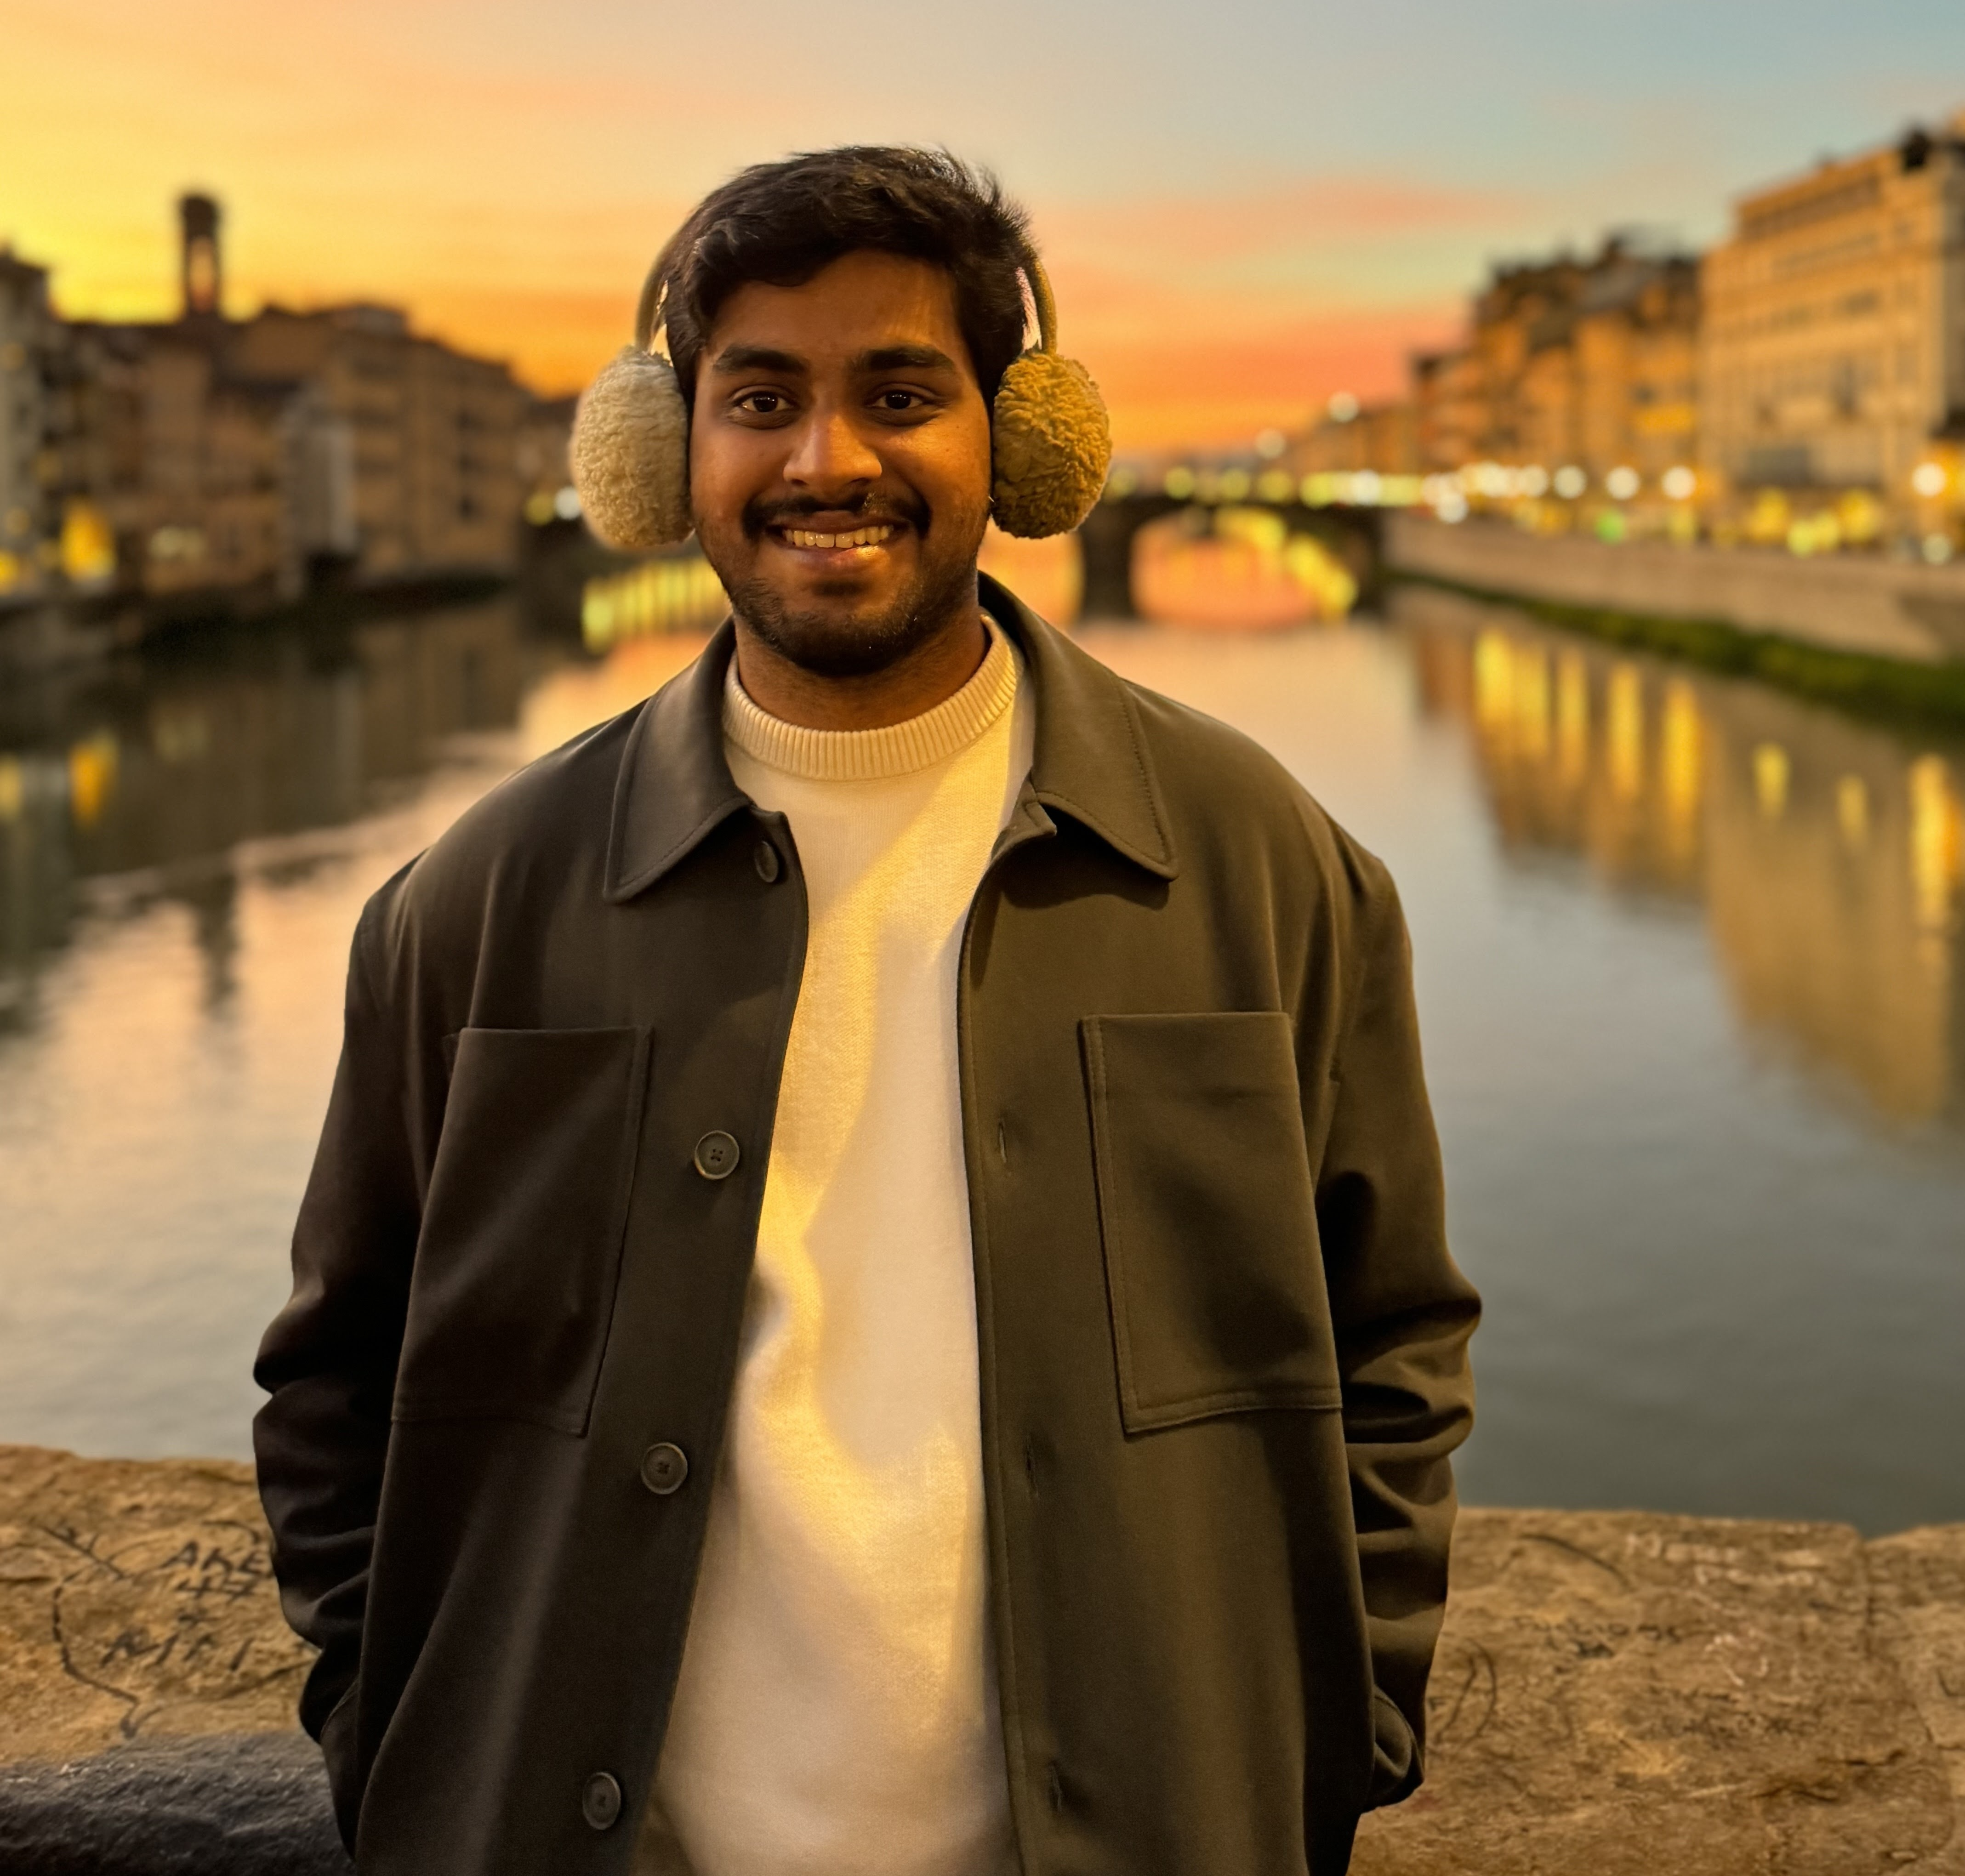
\includegraphics[height=1cm]{images/Shravan_Nayak.jpg}}
                \subfloat[]{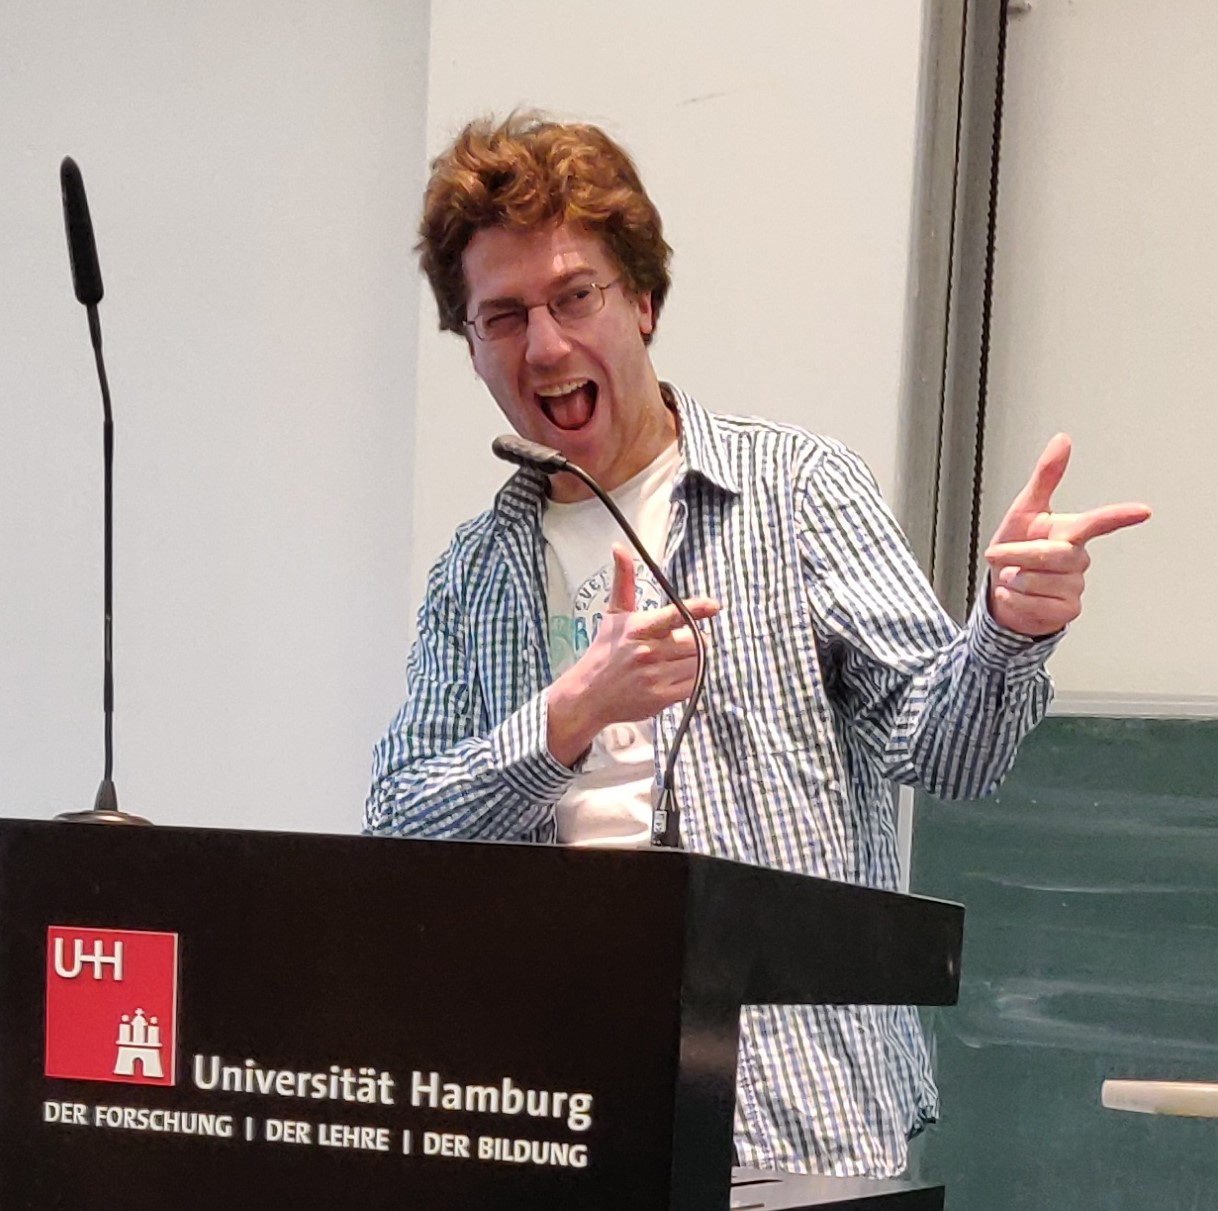
\includegraphics[height=1cm]{images/Christian_Schuler_Lecture.jpg}}
                \subfloat[]{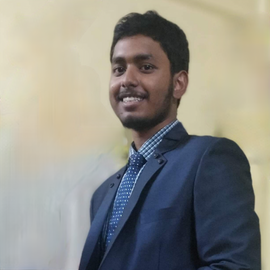
\includegraphics[height=1cm]{images/Debjoy_Saha.png}}
                \subfloat[]{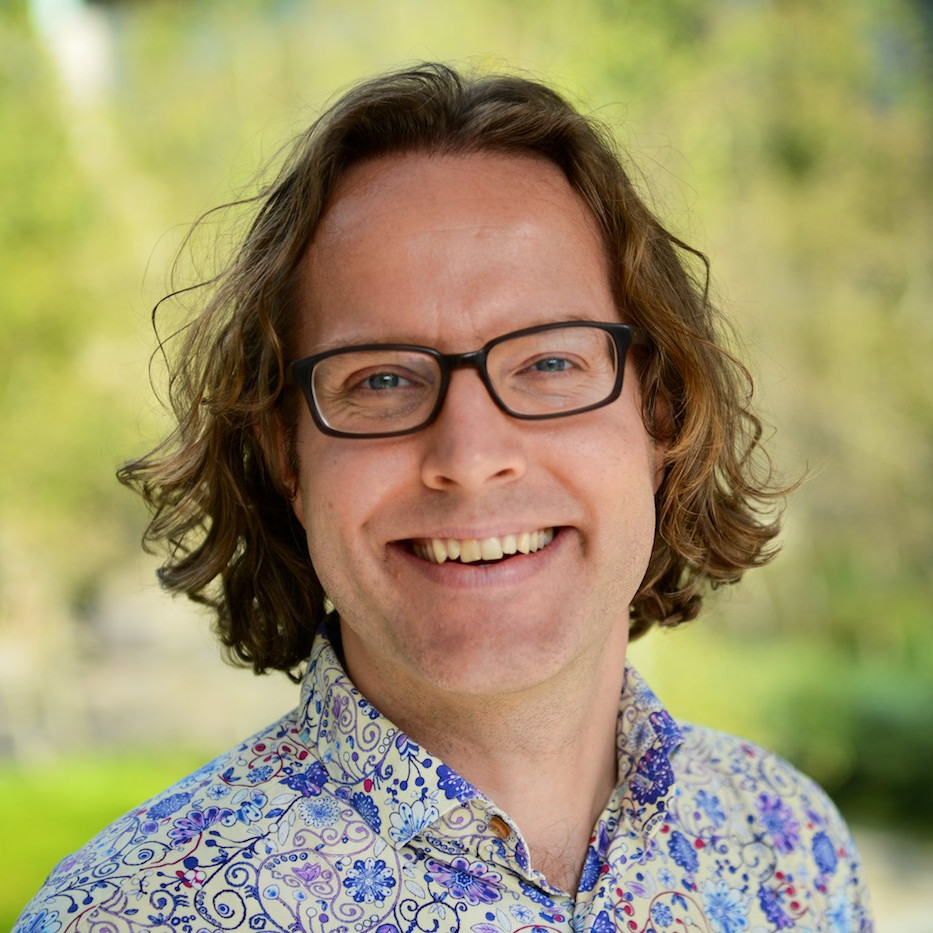
\includegraphics[height=1cm]{images/Timo_Baumann.jpg}}
            \end{figure}
            %\\ Shravan, Christian, Debjoy, Timo
        \end{minipage}
    \end{minipage}
    
    \begin{minipage}{.6\textwidth}
        {\color{thiscolor}$\bullet$} Linux Articles: NLP mit NN \citep{baumann2022NaturalLanguageProcessing} \& Lip-Synched \citep{baumann2023LipSynchedLinuxMagazine}
        % Natural Language Processing mit Neuronalen Netzen & Lip-Synched
        \begin{figure}
        \centering
        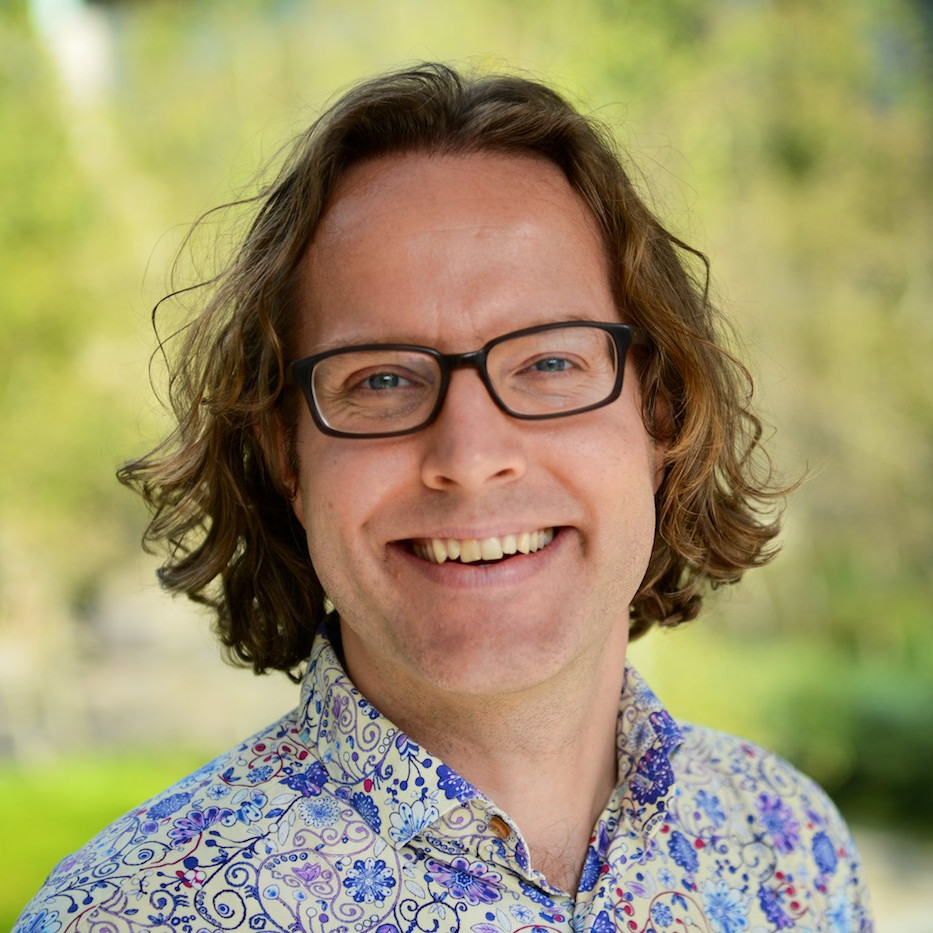
\includegraphics[width=0.2\textwidth]{images/Timo_Baumann.jpg}
        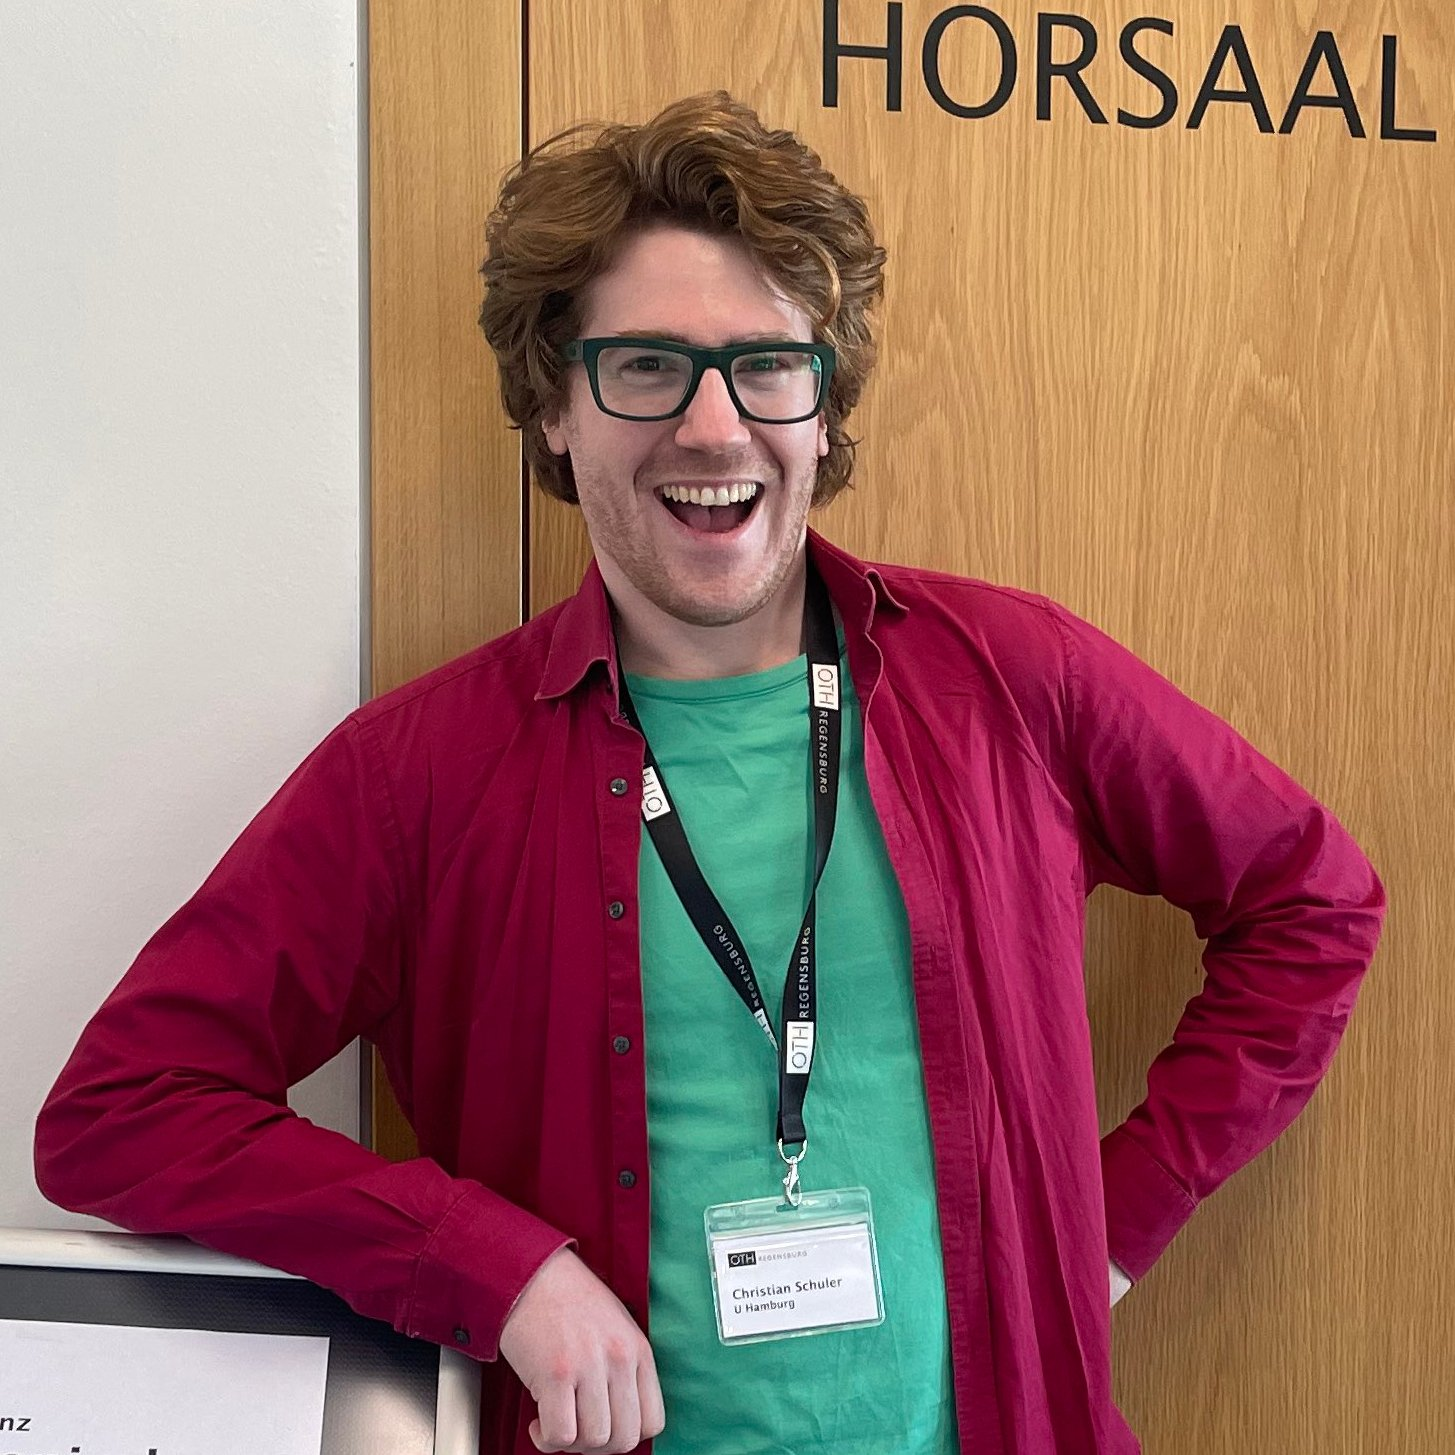
\includegraphics[width=0.2\textwidth]{images/Christian_Schuler_Essv.jpg}
    \end{figure}
    \end{minipage}\hfill%
    \begin{minipage}{.35\textwidth}
        {\color{thiscolor}$\bullet$} StudyToolkitVid
        \begin{figure}
        \centering
        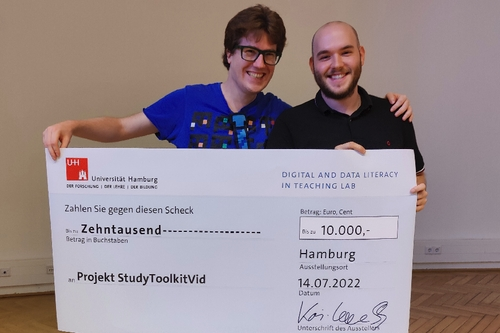
\includegraphics[width=0.8\textwidth]{images/proj-2022-ddlitlab-StudyToolkitVid-500x333.jpg} 
        \end{figure}
    \end{minipage}

    \begin{minipage}{1.0\textwidth}
        \begin{minipage}{.6\textwidth}
            {\color{thiscolor}$\bullet$} Exploration of linguistic information found in \\
            inter-utterance pauses \citep{schuler2024CanWeSee}
            %Can We See Your Response Before You Speak? Exploring Linguistic Information Found in Inter-Utterance Pauses \citep{schuler2024CanWeSee}
            %\vspace{-10mm}
        \end{minipage}
        \begin{minipage}{.4\textwidth}
            \begin{figure}
            \centering
            \captionsetup[subfigure]{labelformat=empty}
                \subfloat[]{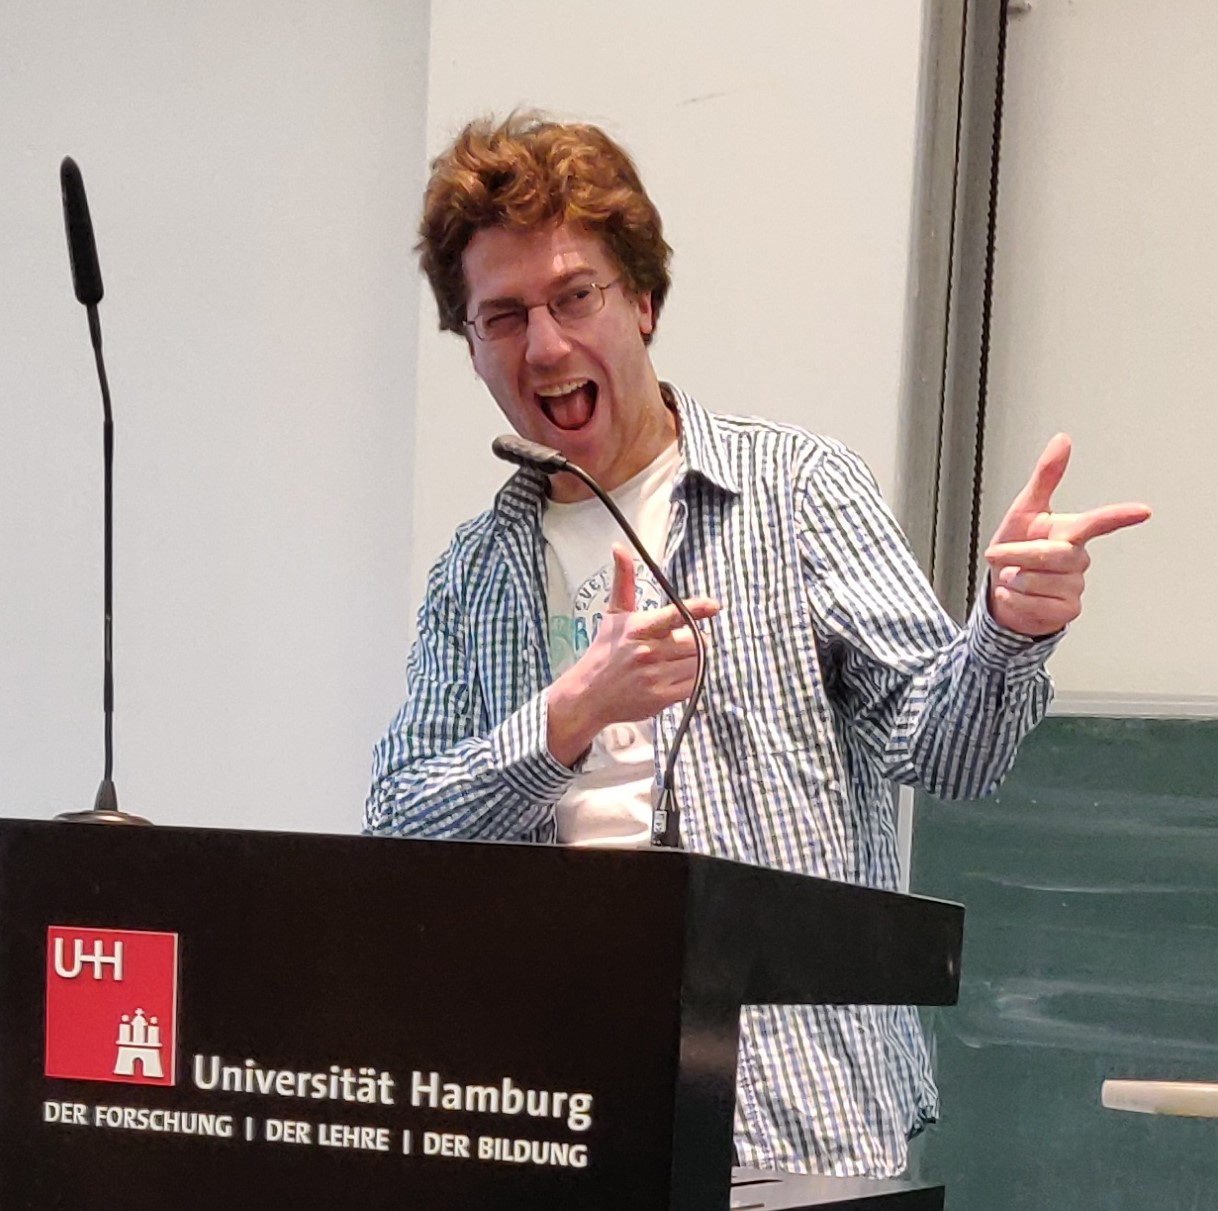
\includegraphics[height=1cm]{images/Christian_Schuler_Lecture.jpg}}
                \subfloat[]{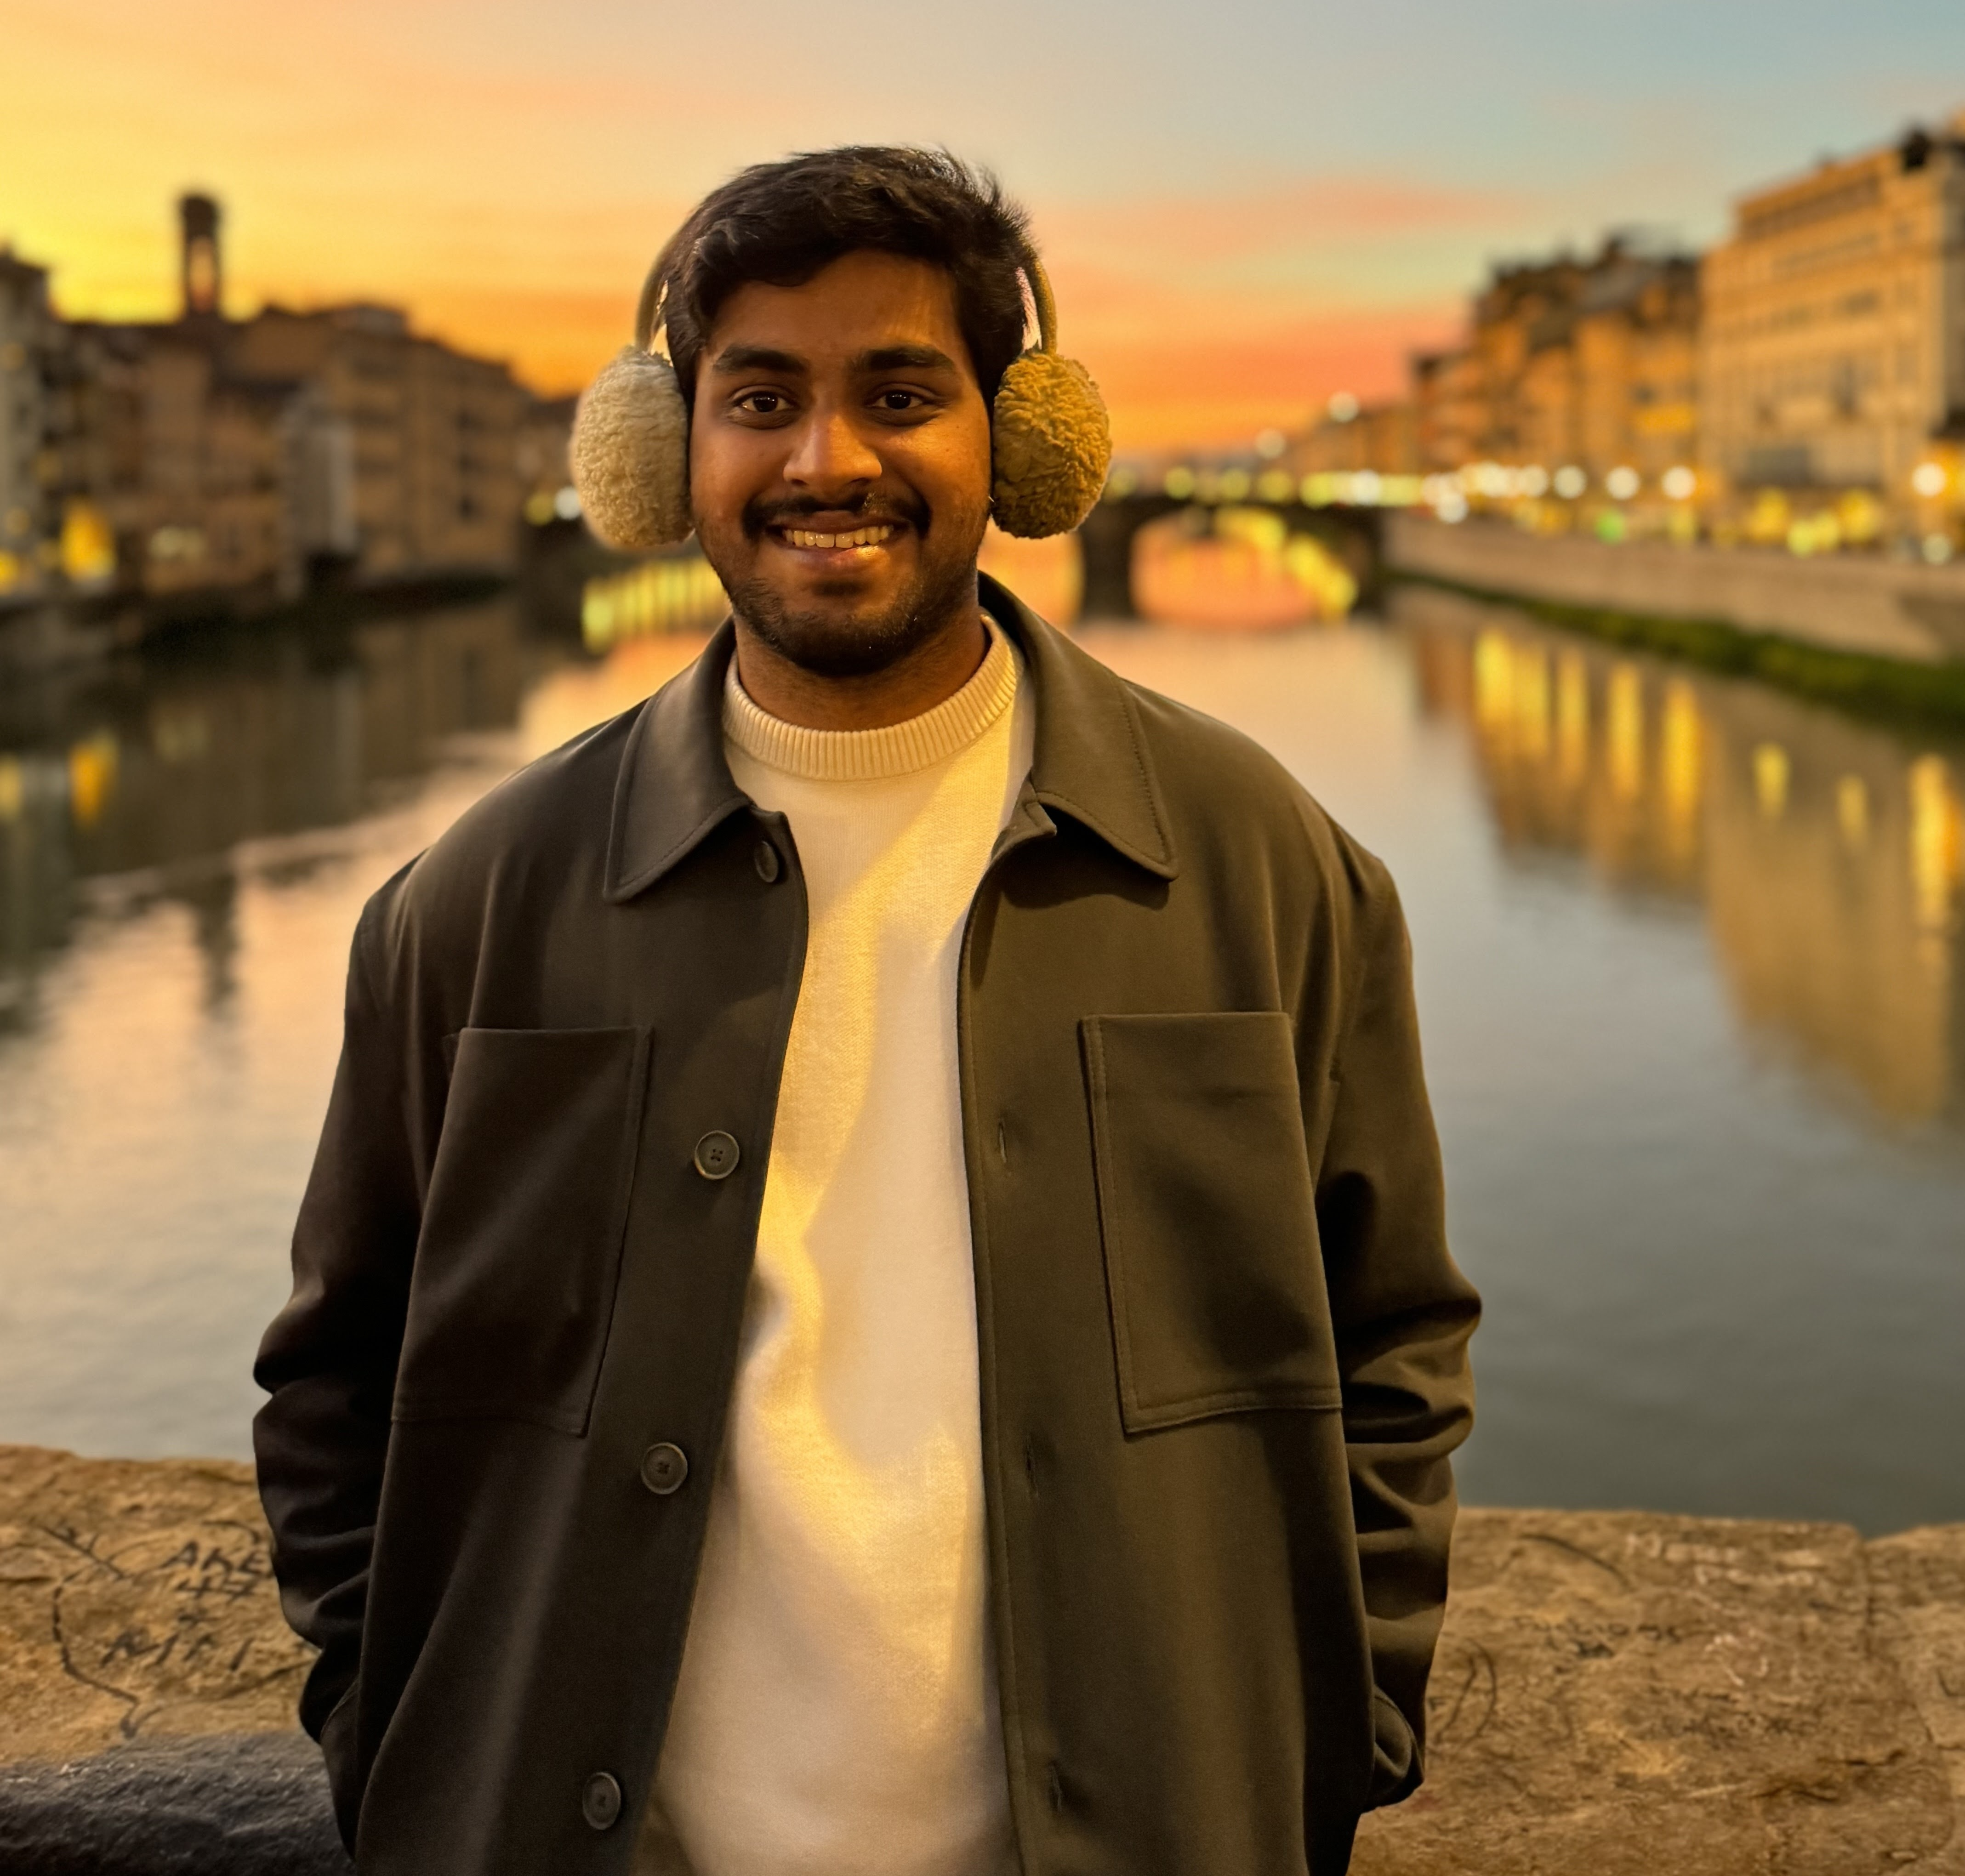
\includegraphics[height=1cm]{images/Shravan_Nayak.jpg}}
                \subfloat[]{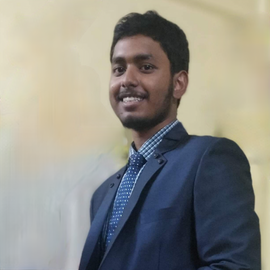
\includegraphics[height=1cm]{images/Debjoy_Saha.png}}
                \subfloat[]{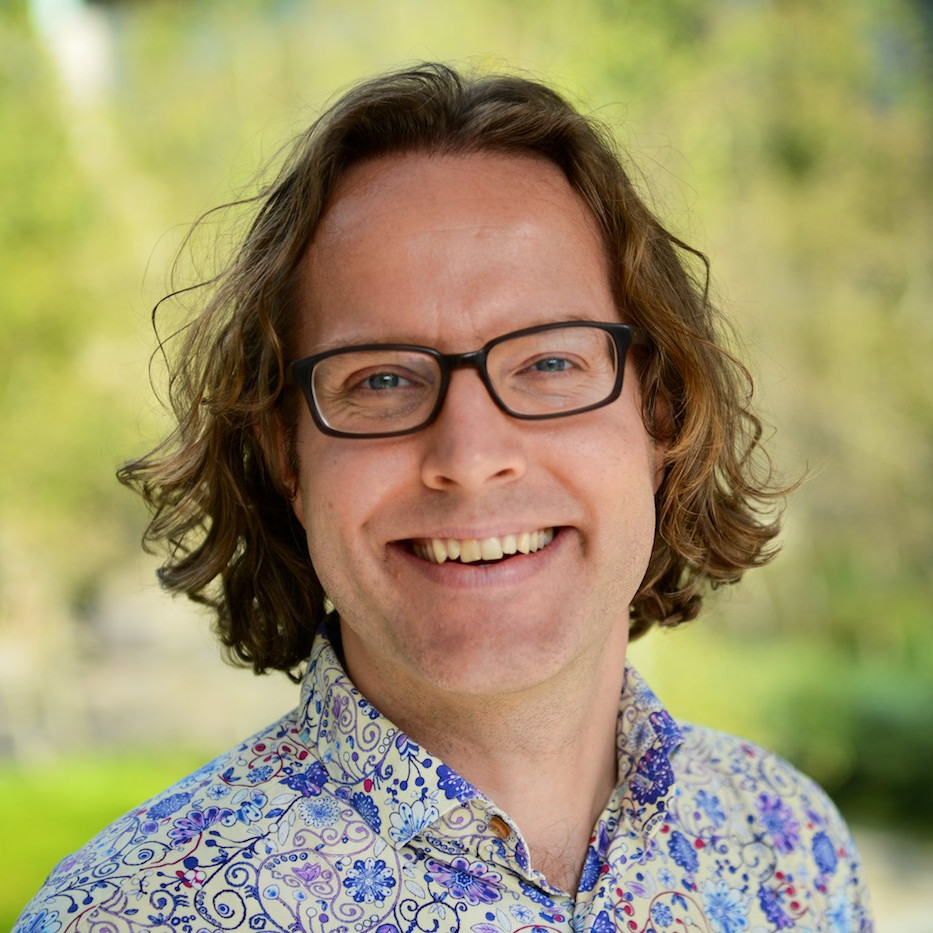
\includegraphics[height=1cm]{images/Timo_Baumann.jpg}}
            \end{figure}
            %\\ Christian, Shravan, Debjoy, Timo
        \end{minipage}
    \end{minipage}
\end{frame}

\begin{frame}[fragile]
	\frametitle{Master's Thesis (2024)}
    {\color{thiscolor}$\bullet$} Title: Leveraging Morphological and Lexical Features in Synthetic Data Generation for Dialect-Specific Machine Translation
    \begin{minipage}{.6\textwidth}
      \begin{figure}
        \centering
        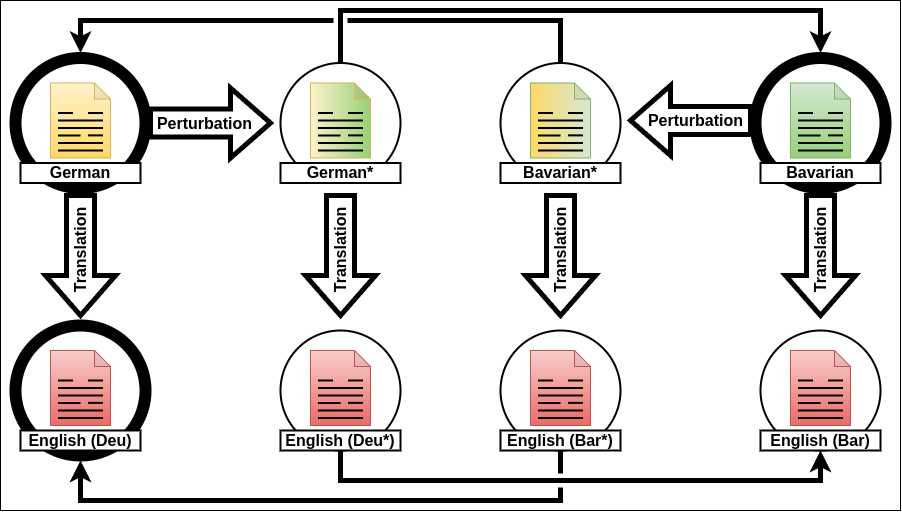
\includegraphics[width=1.0\textwidth]{images/ChameleonMT-MT-ExperimentSetupOverview.png} 
    \end{figure}
    \end{minipage}%
    \begin{minipage}{.4\textwidth}
    \vspace{-4mm}
        \centering
        \begin{figure}
        \centering
        \captionsetup[subfigure]{labelformat=empty}
            \subfloat[Christian Schuler]{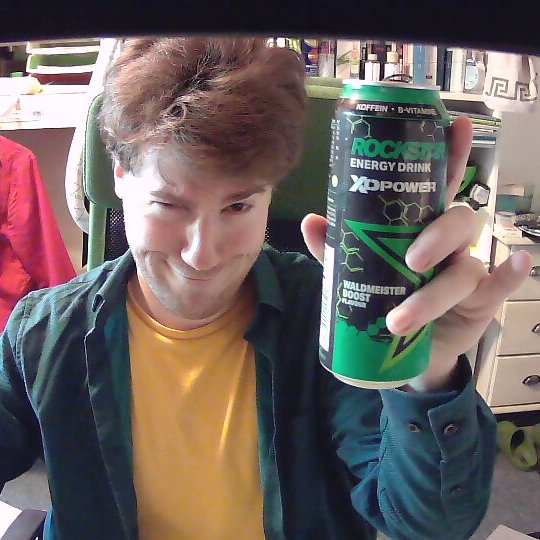
\includegraphics[height=2cm]{images/Christian_Schuler_Energydrink.jpg}}
            \subfloat[Dr. Sina Ahmadi]{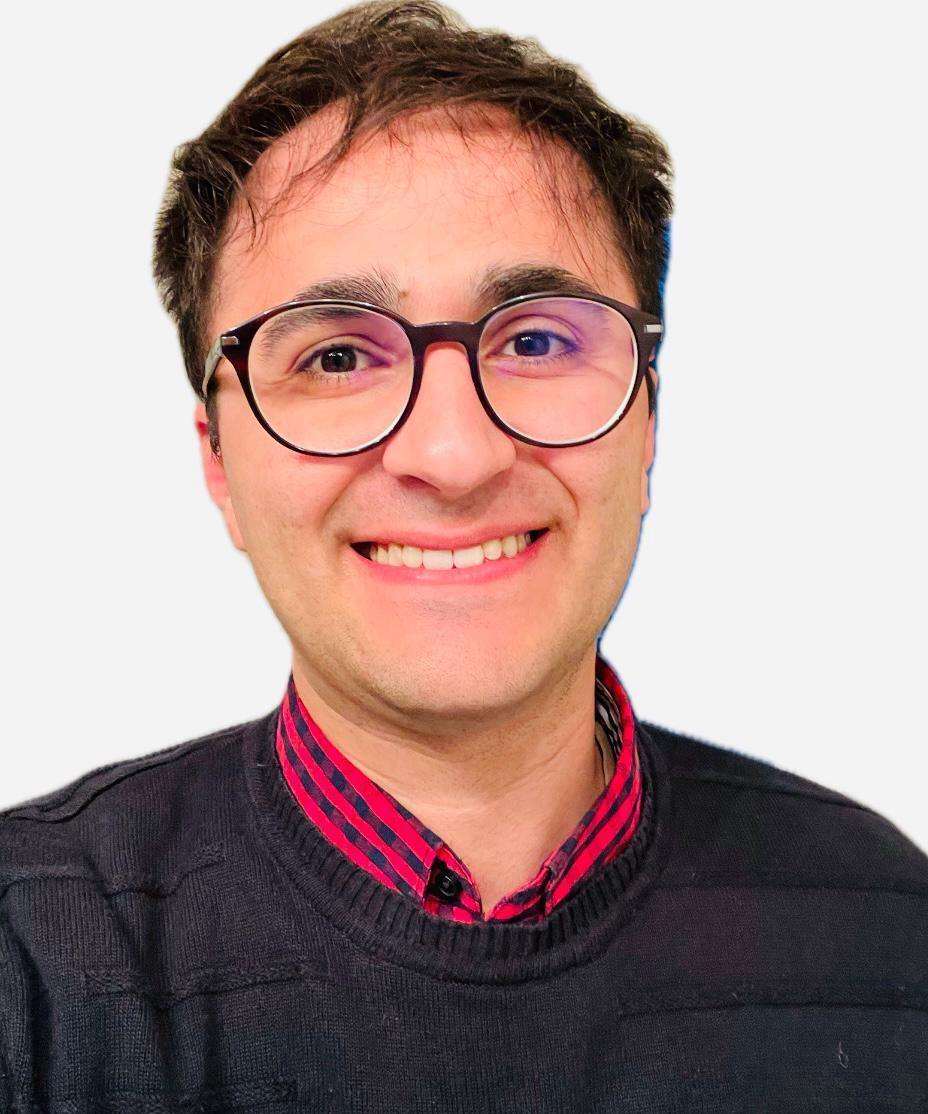
\includegraphics[height=2cm]{images/Sina_Ahmadi.jpg}}\\
            \subfloat[Dr. Seid Muhie Yimam]{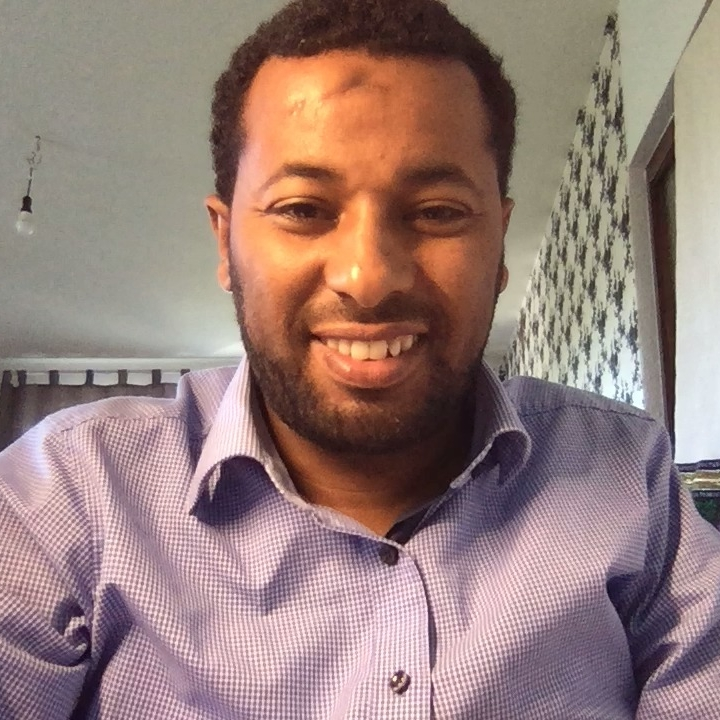
\includegraphics[height=2cm]{images/Seid_Muhie_Yimam.jpeg}}
            \subfloat[Prof. Chris Biemann]{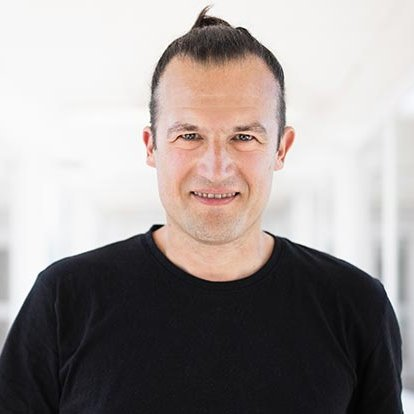
\includegraphics[height=2cm]{images/Chris_Biemann.jpg}}
        \end{figure}
    \end{minipage}
   \end{frame}

\begin{frame}[fragile]
	\frametitle{Master's Thesis Build-up (2023-2024)}
    \begin{minipage}{.49\textwidth}
        {\color{thiscolor}$\bullet$} Towards a Complete Mapping of Kurdish Dialectology \citep{schuler2023CompleteMappingKurdish}
        \begin{center}
            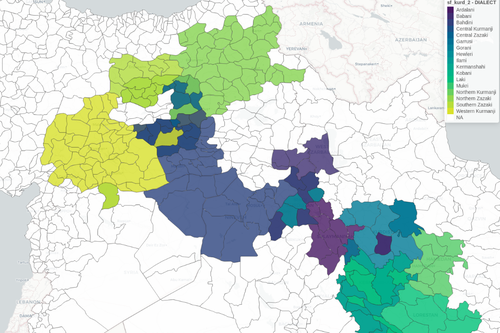
\includegraphics[height=2.5cm]{images/ickl6_dialectmapping.png}
            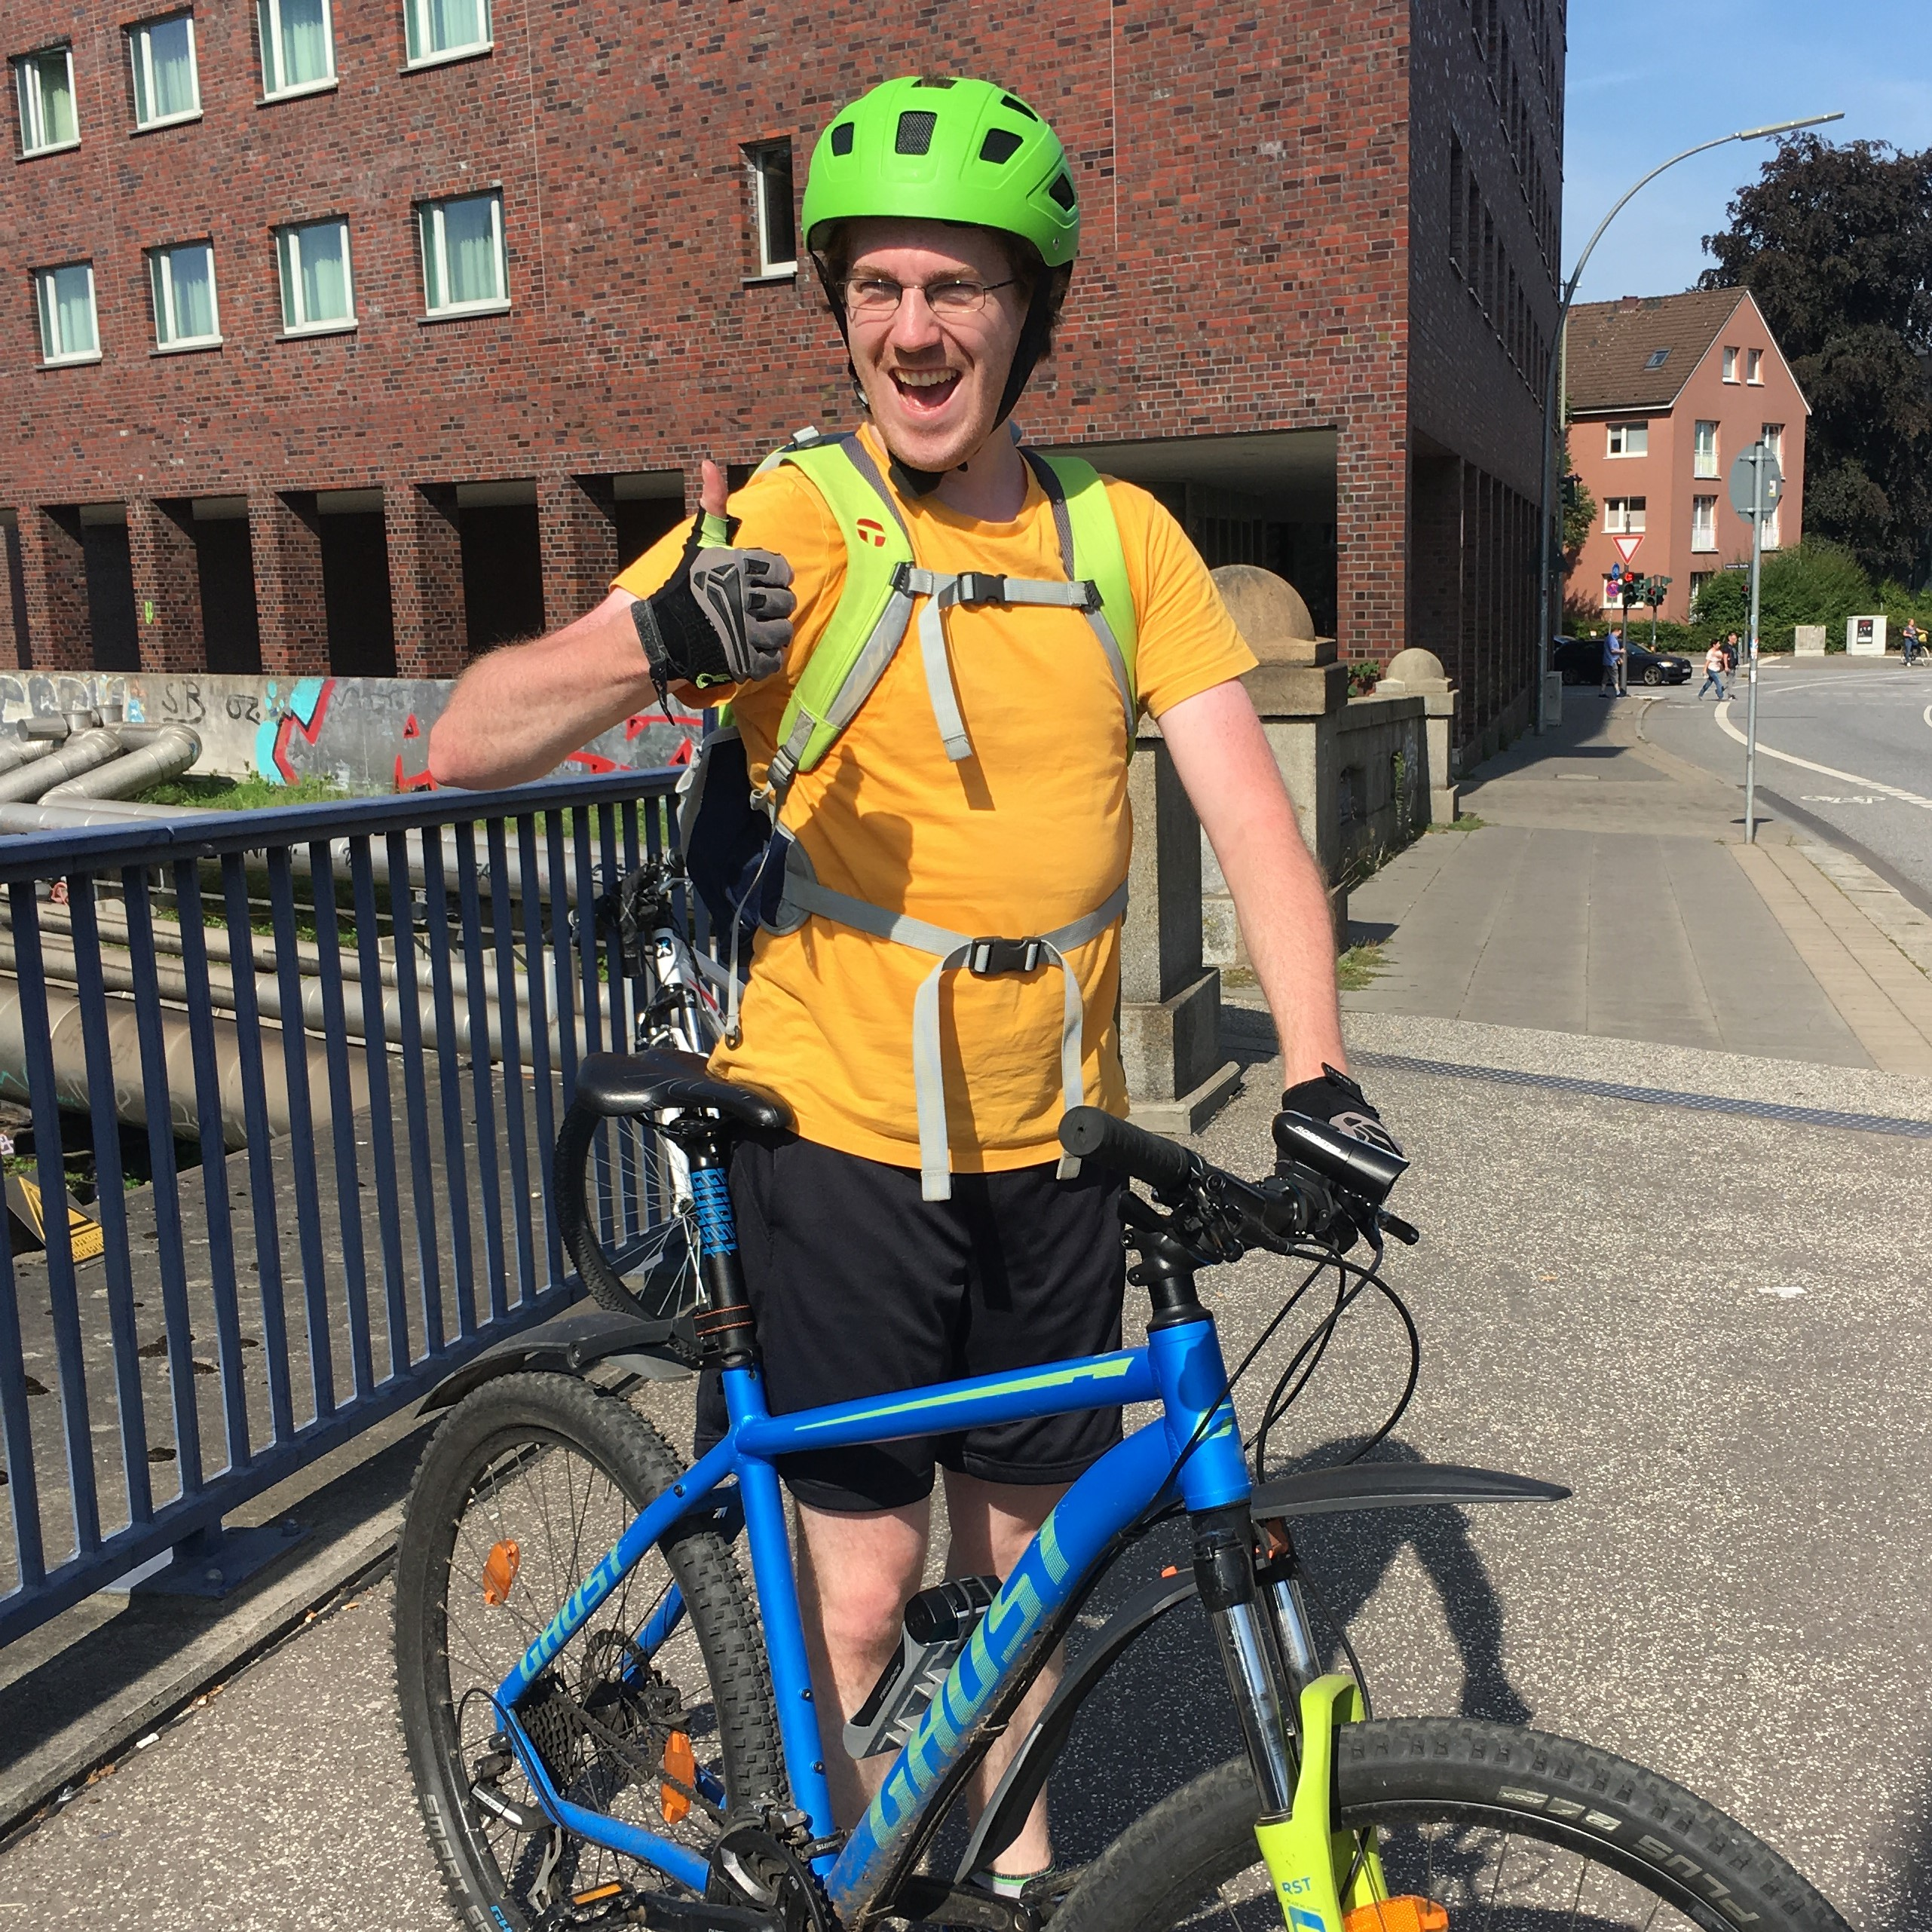
\includegraphics[height=1.2cm]{images/Christian_Schuler_Bike.JPG} 
            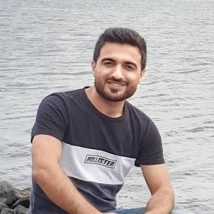
\includegraphics[height=1.2cm]{images/Raman_Ahmad.png} 
        \end{center}
    \end{minipage}\hfill%
    \begin{minipage}{.49\textwidth}
        {\color{thiscolor}$\bullet$} Analysis of Phonology and Morphology in the Kobani Dialect \citep{ahmad2023AnalysisPhonologyMorphology}
        \begin{center}
            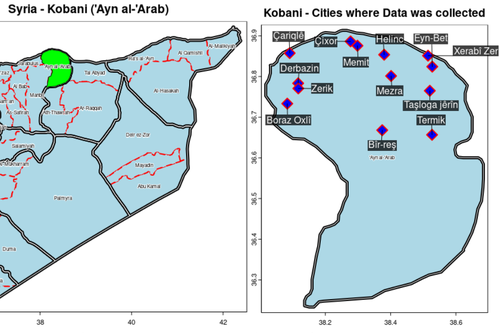
\includegraphics[height=2.5cm]{images/ickl6_kobanianalysis.png}
            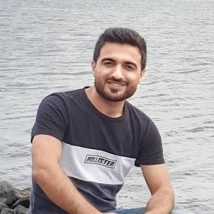
\includegraphics[height=1.2cm]{images/Raman_Ahmad.png} 
            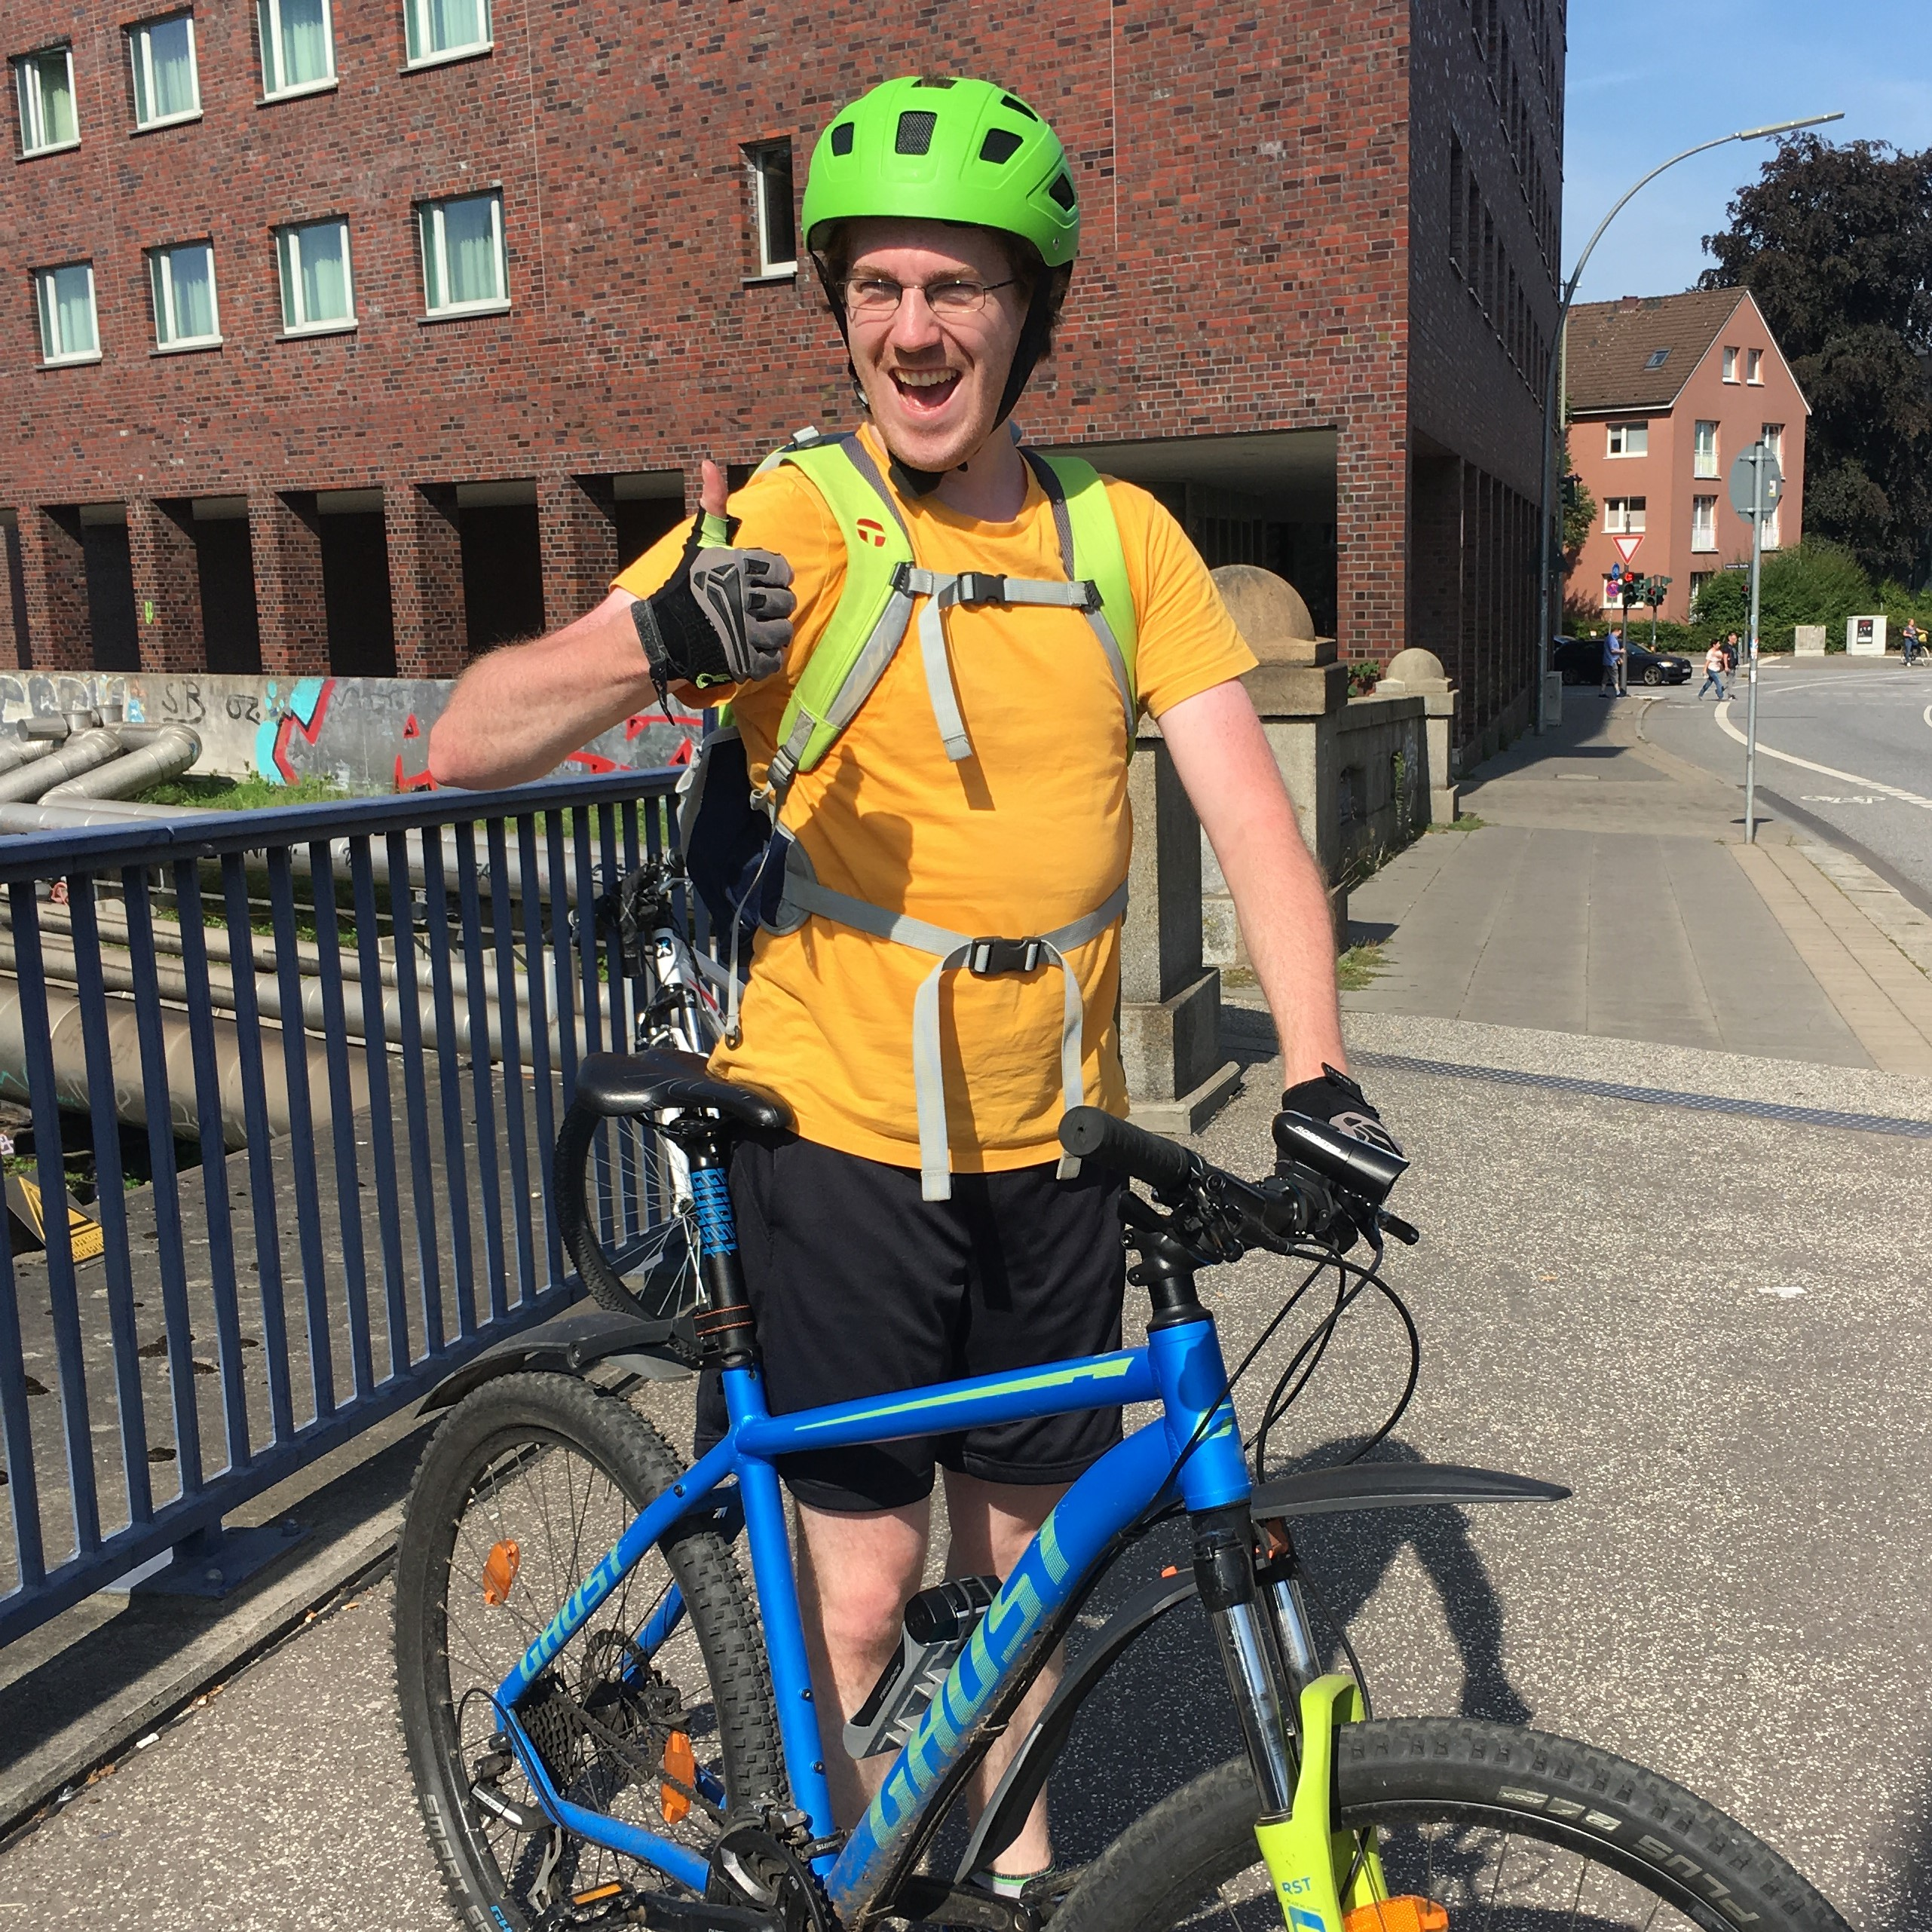
\includegraphics[height=1.2cm]{images/Christian_Schuler_Bike.JPG} 
        \end{center}
    \end{minipage}

    \vspace{1cm}
    \begin{minipage}{1.0\textwidth}
    \centering
    {\color{thiscolor}$\bullet$} MTACR - Multilingual Text As Corpus Repository
    %
\includegraphics[height=1.5cm]{images/TextAsCorpusRep-Auxiliary-Logo.png}
    \end{minipage}
\end{frame}

\section{Introduction\&Motivation}
\begin{frame}[fragile]
	\frametitle{Project Team}
    \captionsetup[subfigure]{labelformat=empty}
    \begin{figure}
        \centering
        \subfloat[]{
\includegraphics[height=1.5cm]{images/TextAsCorpusRep-Auxiliary-Logo.png}}\\
        Multilingual Text As Corpus Repository\\
        \subfloat[Christian Schuler]{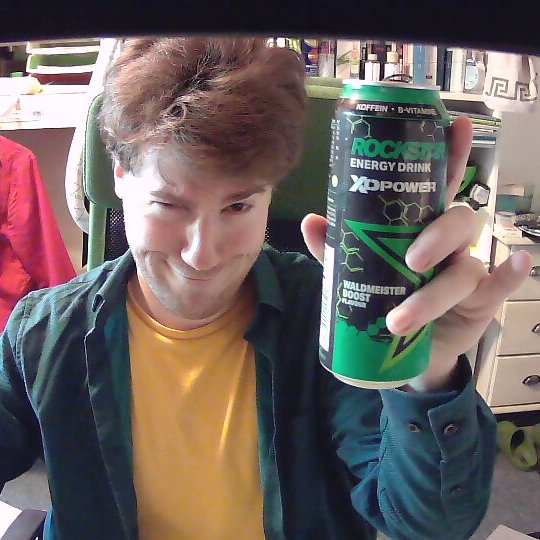
\includegraphics[height=2cm]{images/Christian_Schuler_Energydrink.jpg}}\hfill
        \subfloat[Tramy Thi Tran]{
\includegraphics[height=2cm]{images/Tramy_Thi_Tran.jpeg}}\hfill
        \subfloat[Deepesha Saurty]{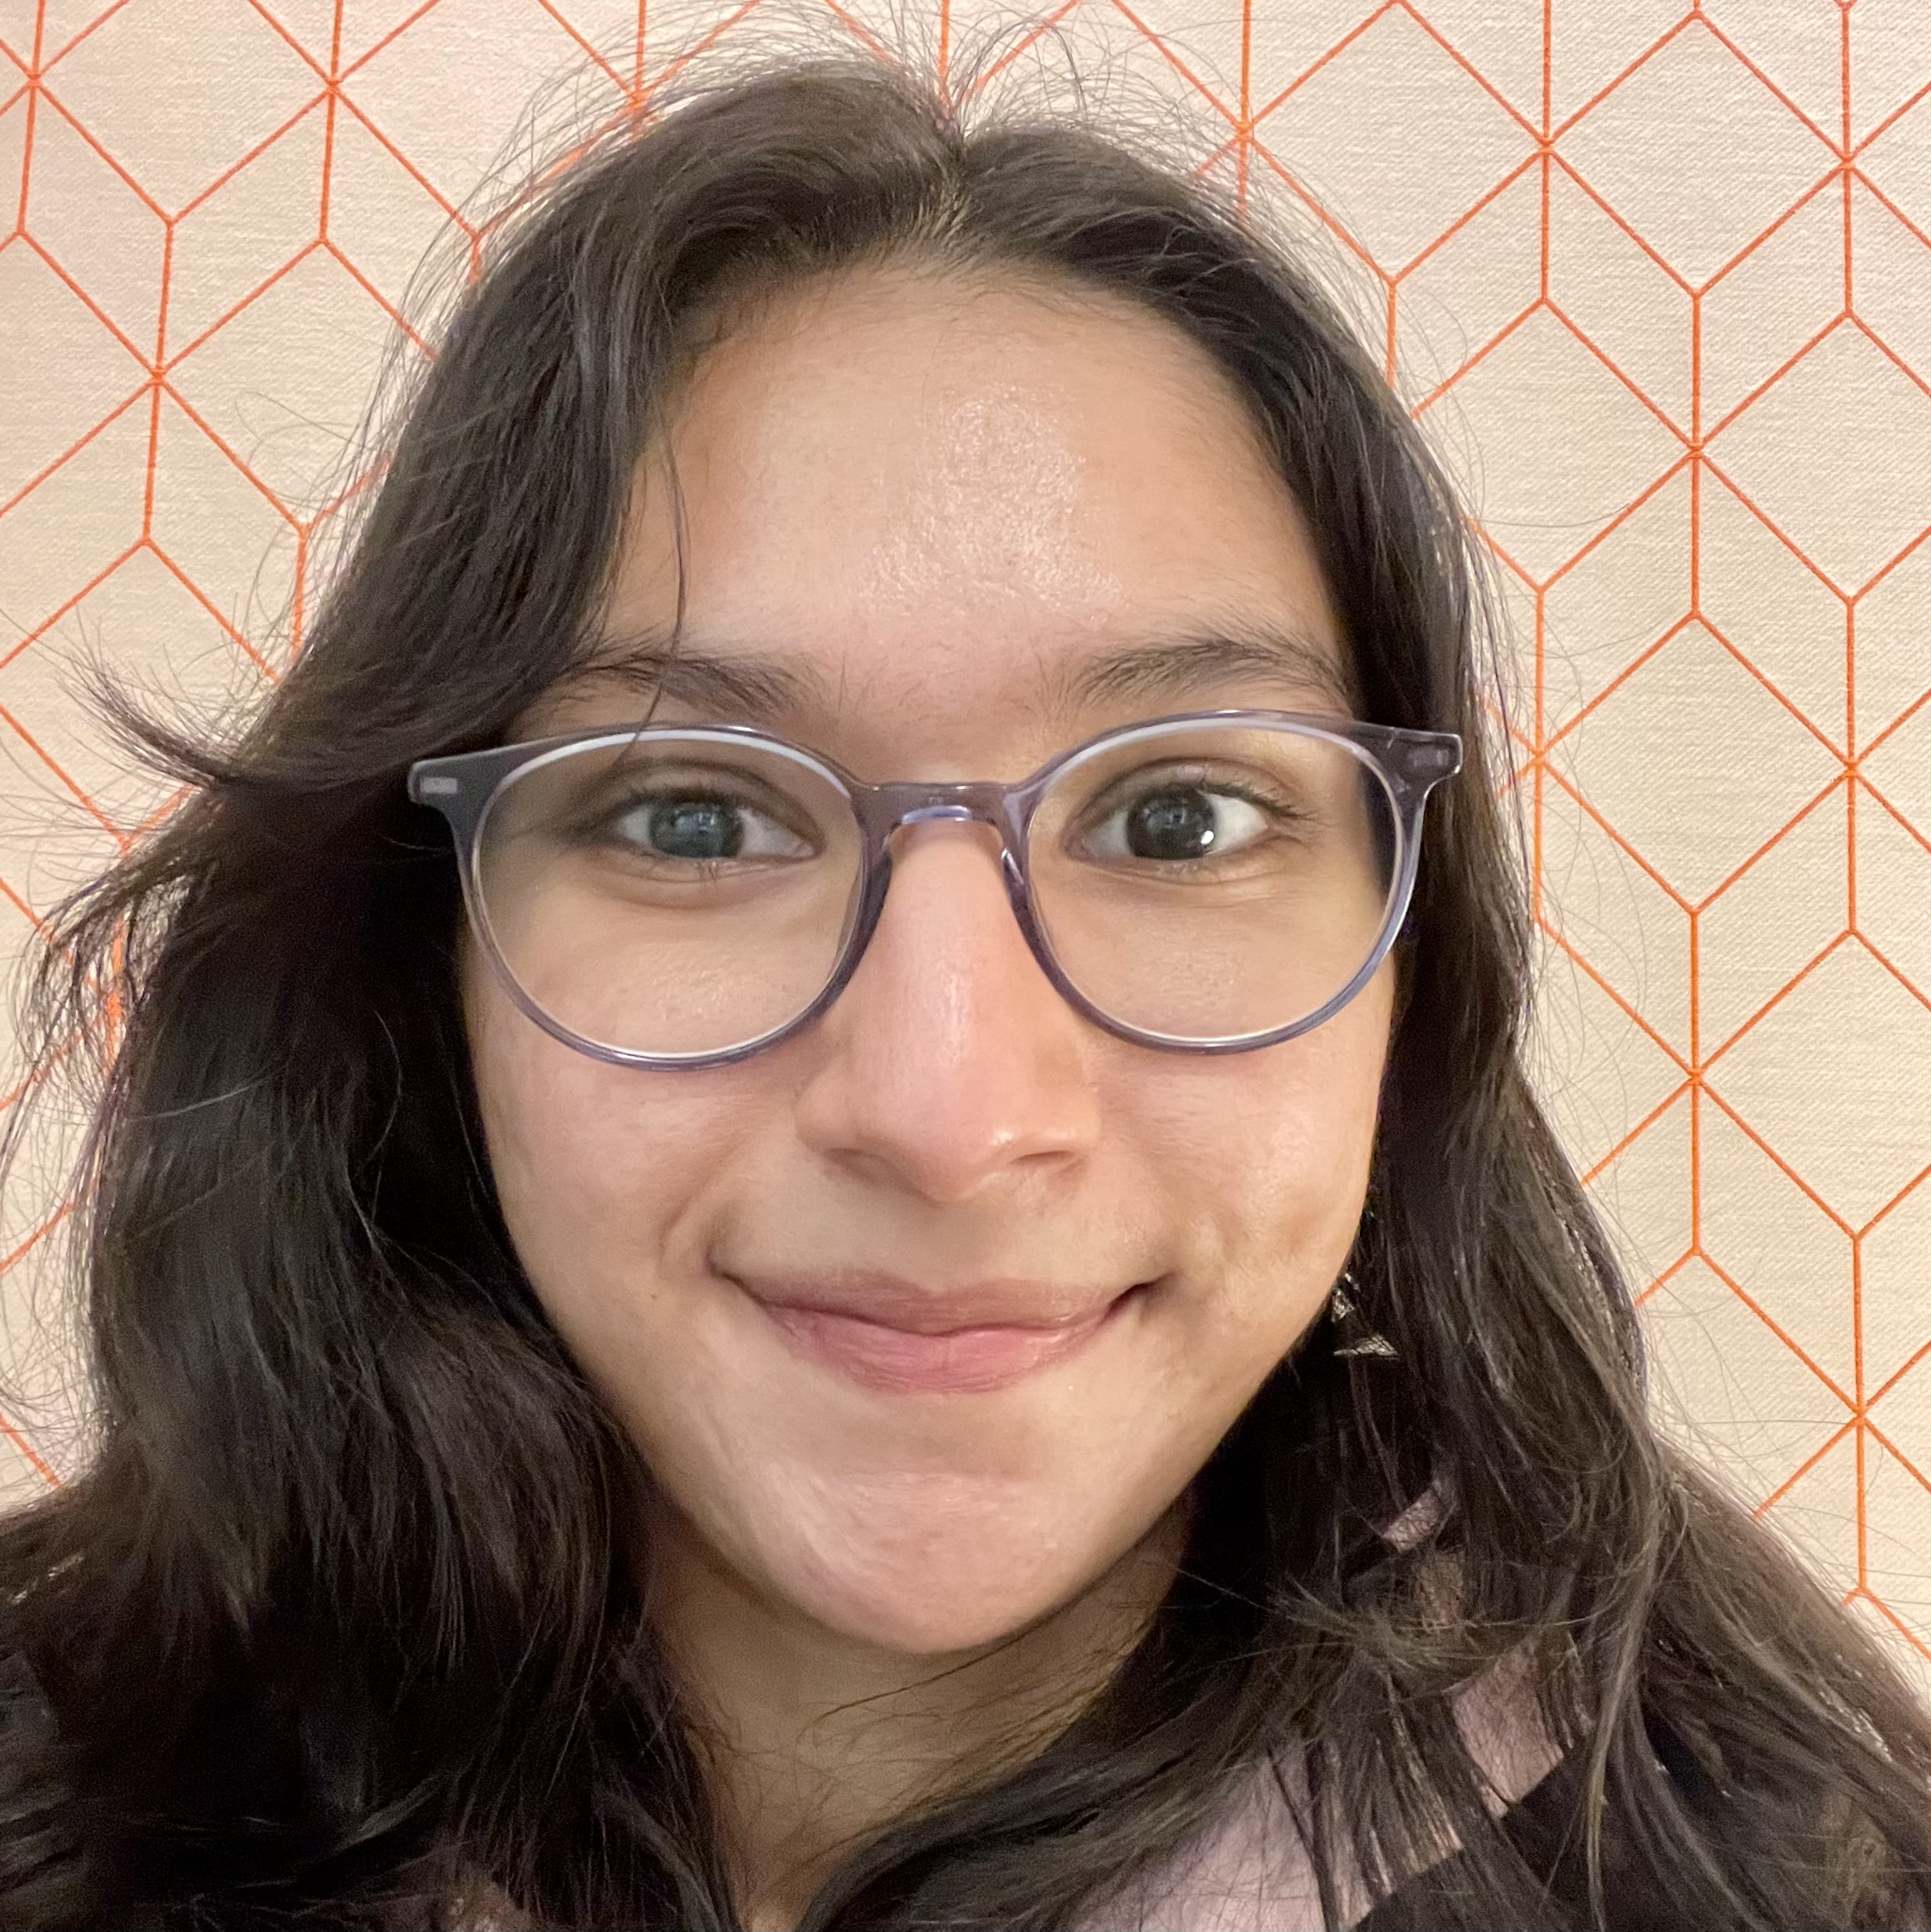
\includegraphics[height=2cm]{images/Deepesha_Saurty.jpg}}\hfill
        \subfloat[Anran Wang]{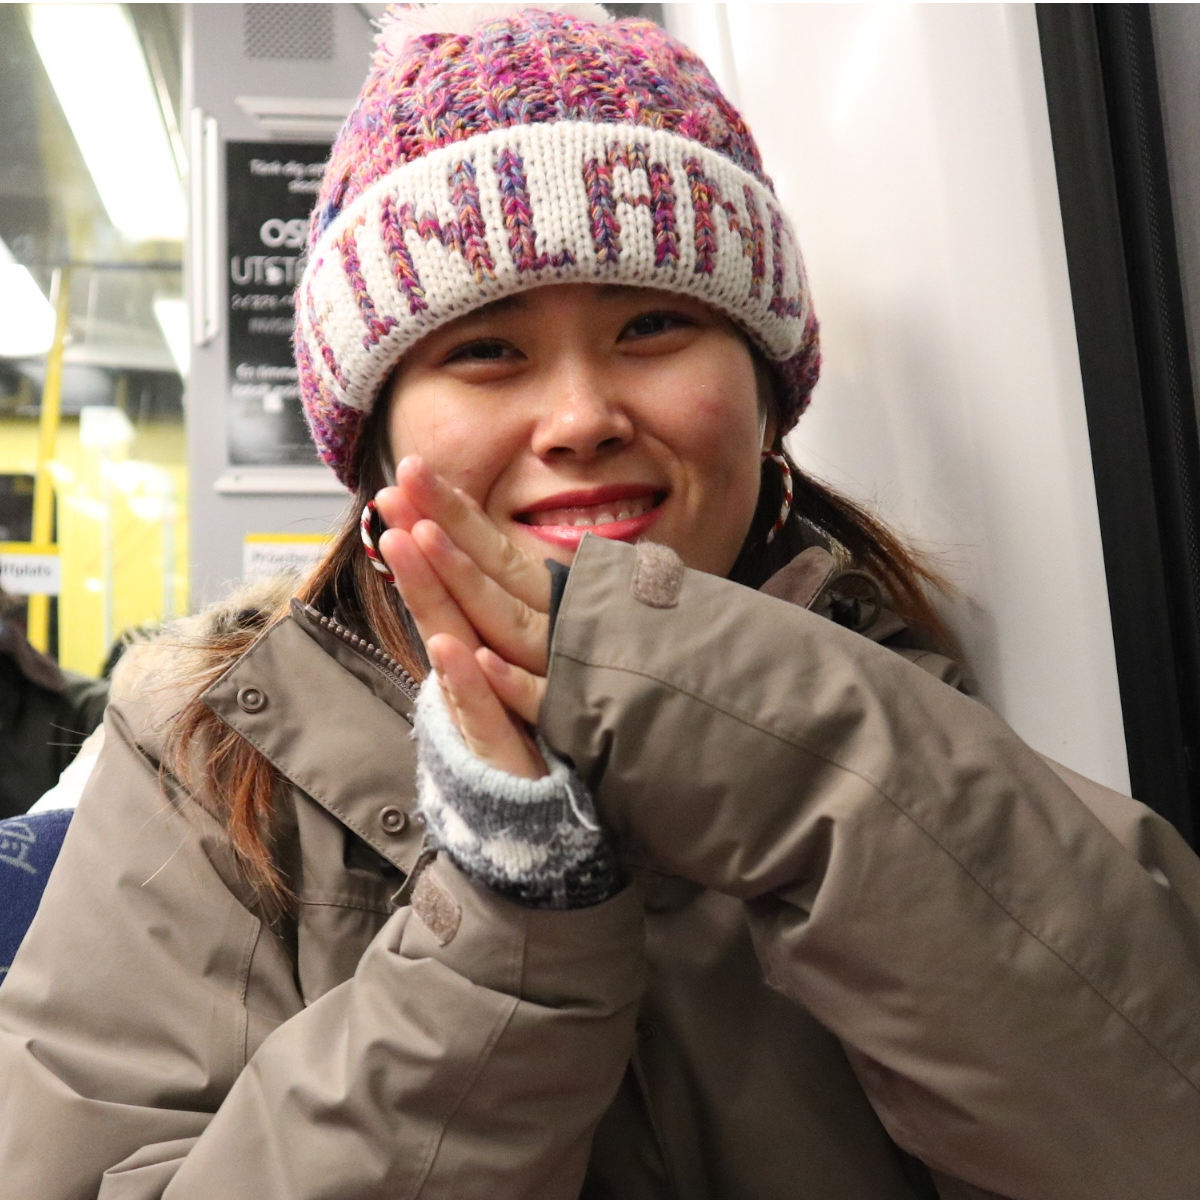
\includegraphics[height=2cm]{images/Anran_Wang.png}}\hfill
        \subfloat[Raman Ahmad]{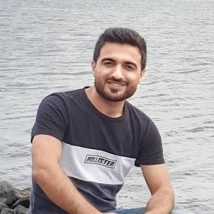
\includegraphics[height=2cm]{images/Raman_Ahmad.png}}\hfill
        \subfloat[Seid Muhie Yimam]{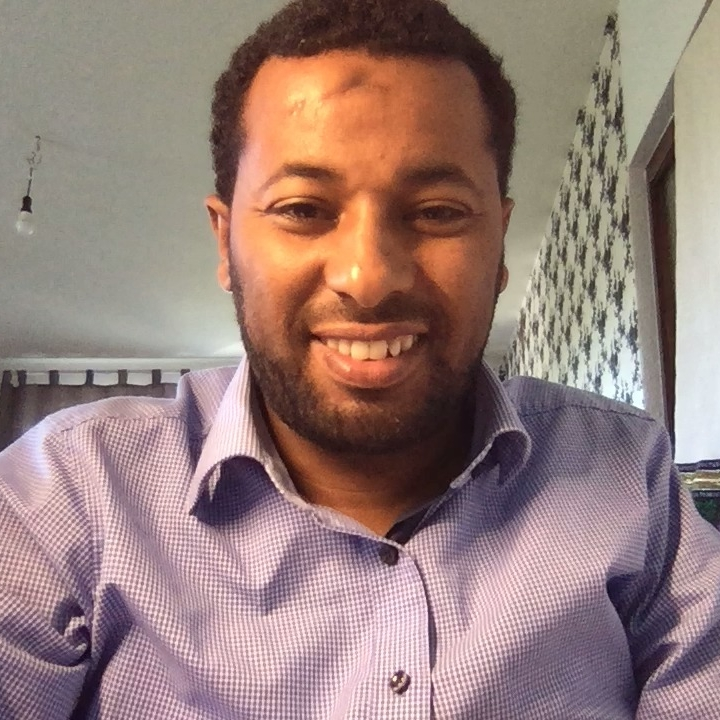
\includegraphics[height=2cm]{images/Seid_Muhie_Yimam.jpeg}}\\
        \subfloat[]{
\includegraphics[width=2cm]{images/uhh-logo.png}}\hfill
        \subfloat[]{
\includegraphics[width=2cm]{images/uhh-logo.png}}\hfill
        \subfloat[]{
\includegraphics[width=2cm]{images/uhh-logo.png}}\hfill
        \subfloat[]{\hspace{.4cm}
\includegraphics[width=1.2cm]{images/tum-logo.png}\hspace{.4cm}}\hfill
        \subfloat[]{
\includegraphics[width=2cm]{images/haw-logo.png}}\hfill
        \subfloat[]{
\includegraphics[width=2cm]{images/uhh-logo.png}}\hfill
    \end{figure}
\end{frame}

\begin{frame}[fragile]
	\frametitle{Translation Systems (Here Google Translate) Failing Languages}
    \begin{figure}
	    \centering
	    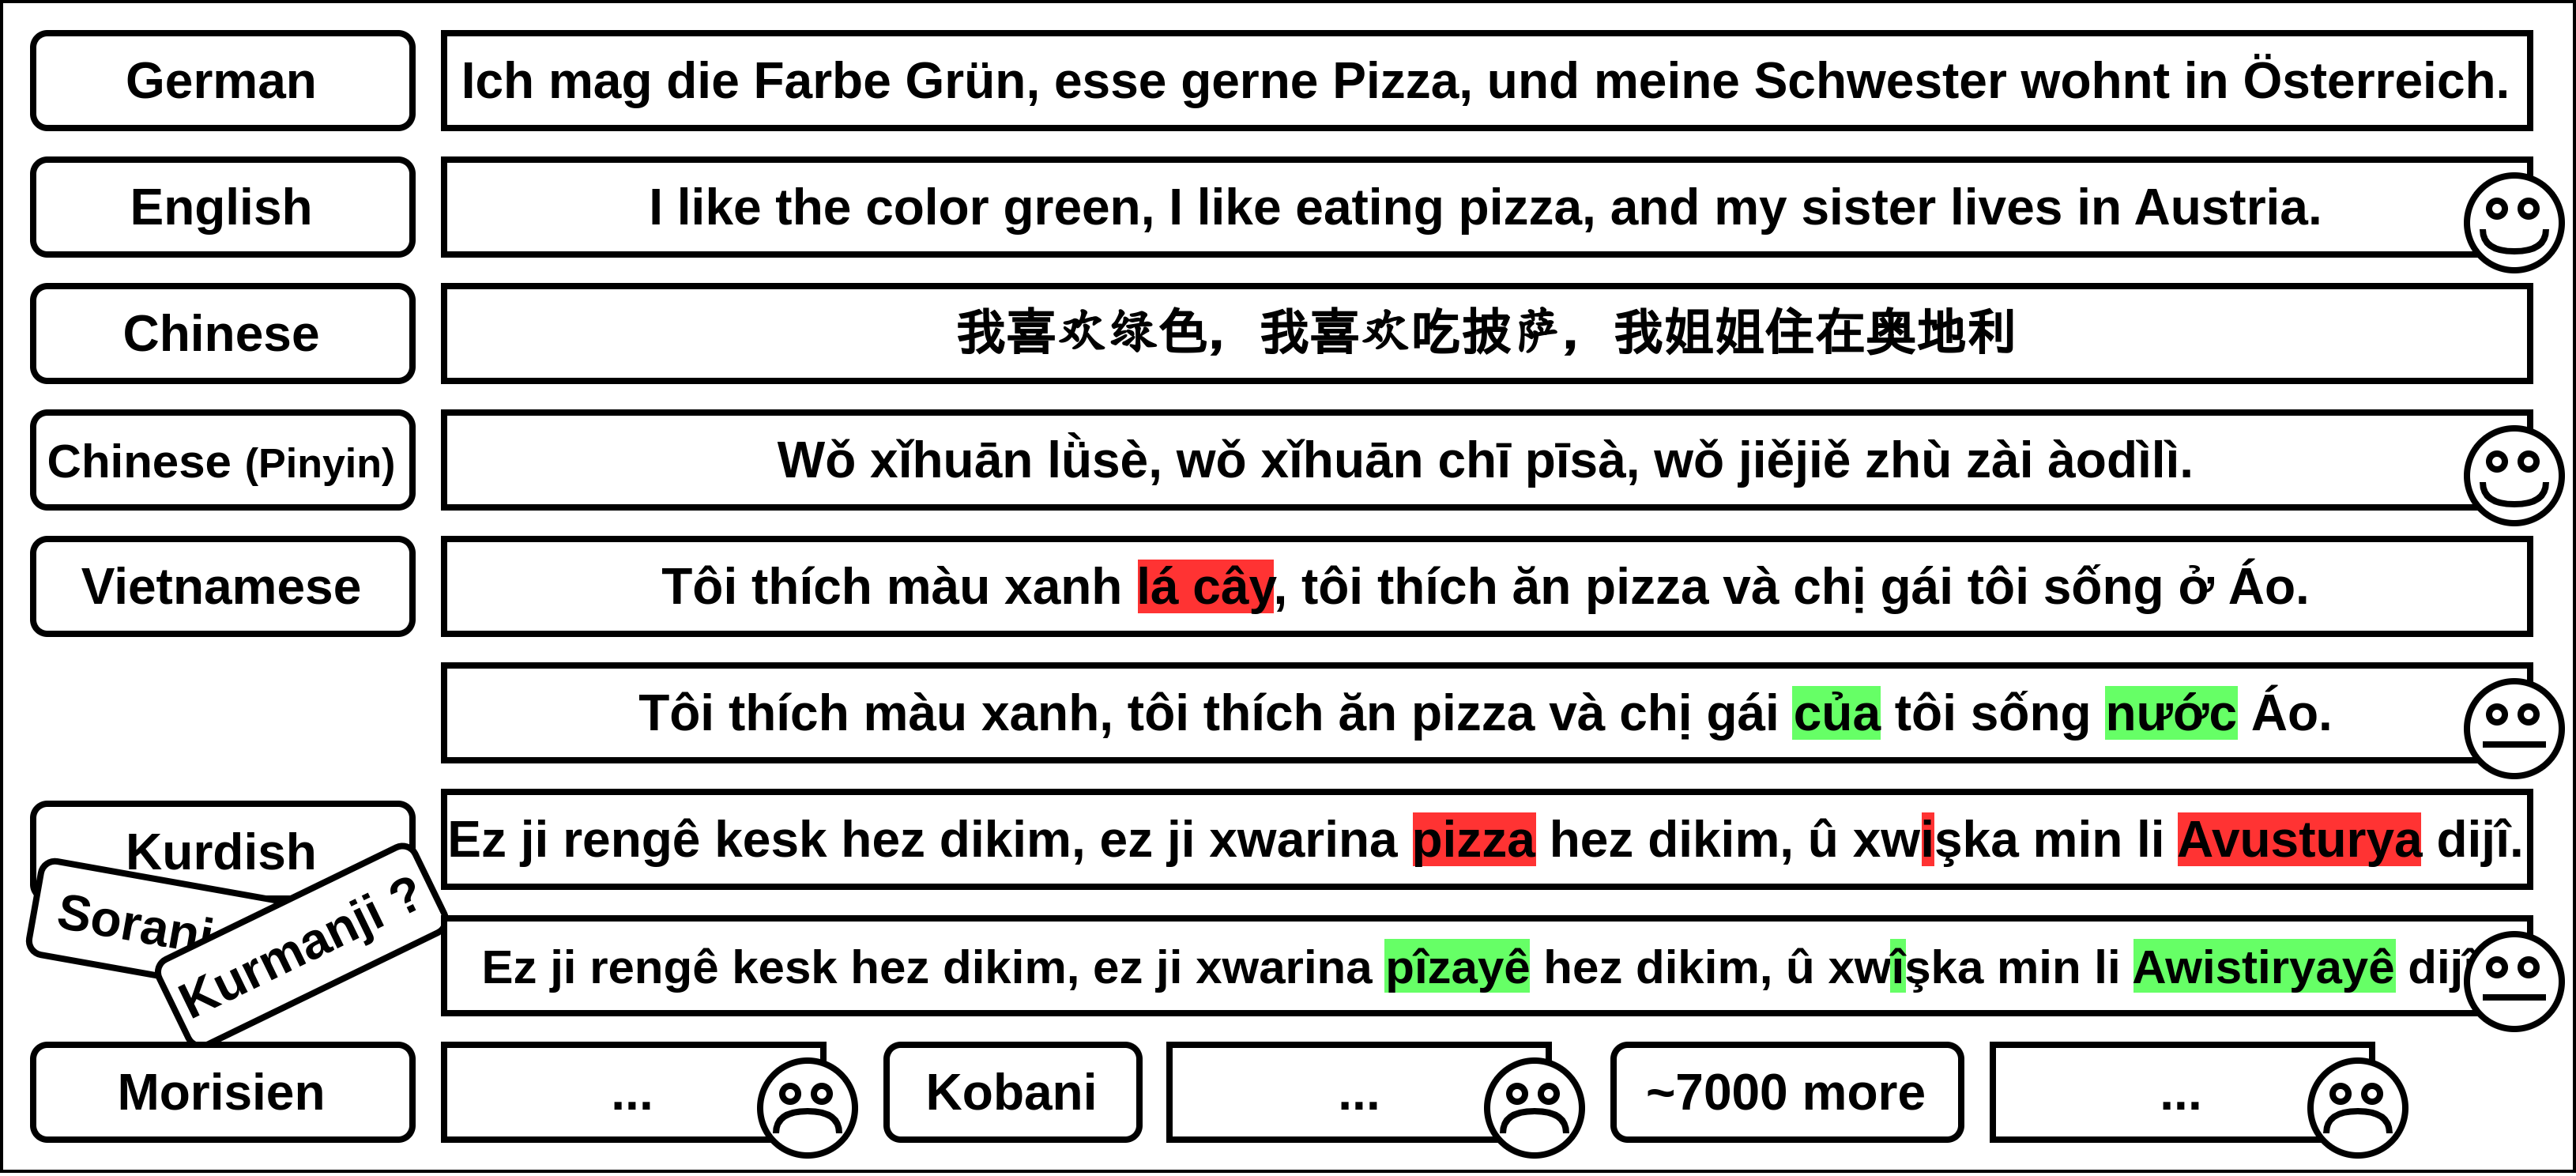
\includegraphics[width=1.0\textwidth]{images/CRAMT-Tool-MotivationSimpleMore.png}
	\end{figure}
\end{frame}

\begin{frame}[fragile]
	\frametitle{Our Goal \& Our Enemies}
	\begin{minipage}{.49\textwidth}
    \begin{figure}
	    \centering
	    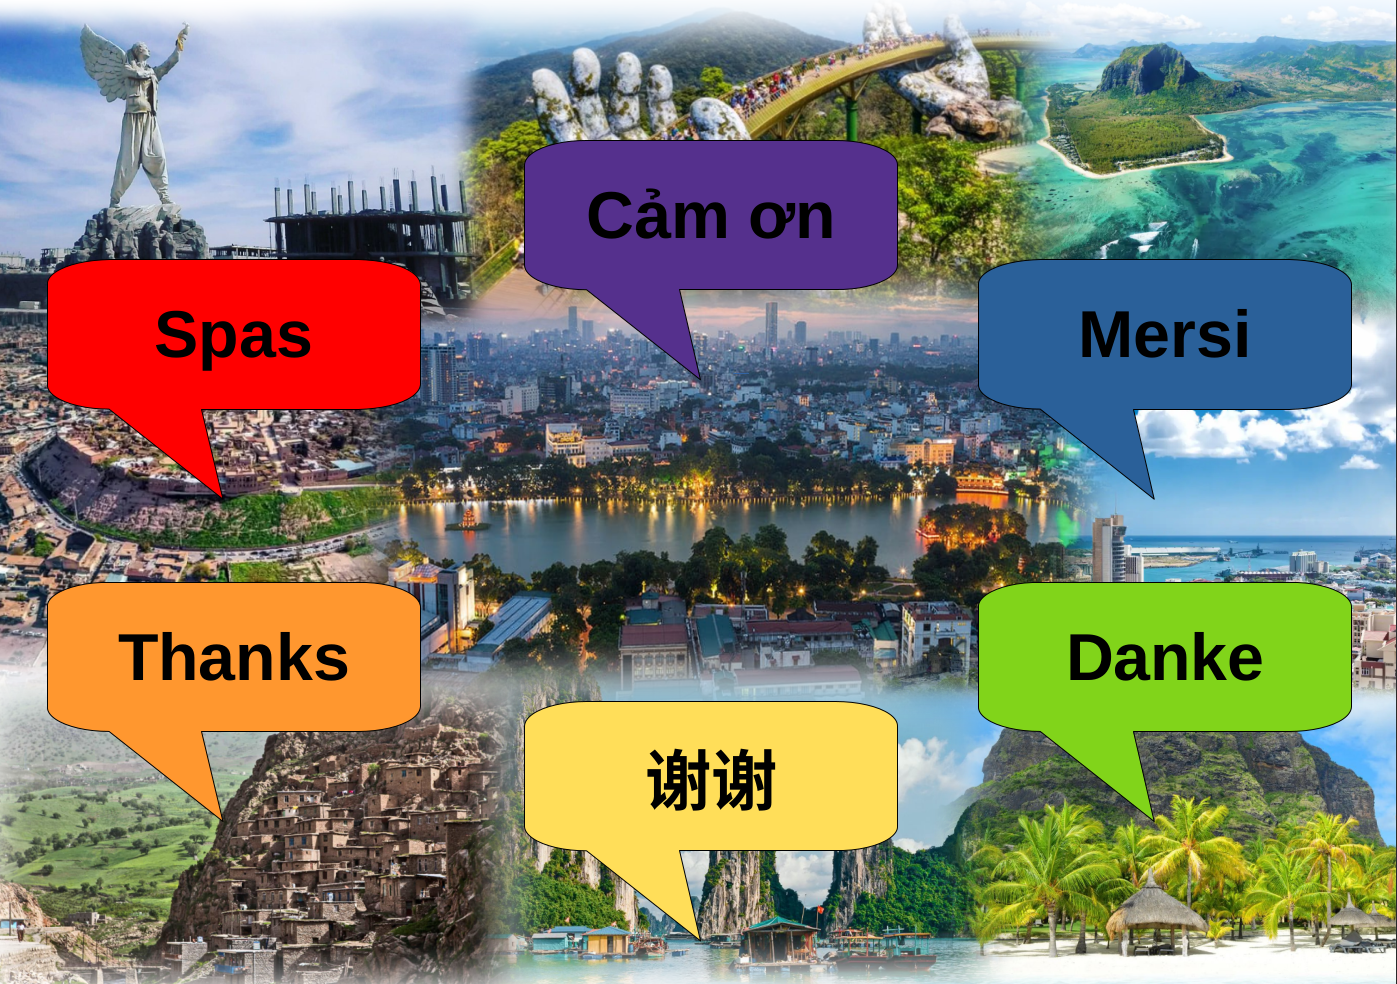
\includegraphics[width=1.0\textwidth]{images/title-banner.png}
	\end{figure}
	\end{minipage}
	\begin{minipage}{.49\textwidth}
	\begin{enumerate}
		\item Time
		\item Bureaucracy
		\item Expert translators (?!)
	\end{enumerate}
	\end{minipage}
\end{frame}


\section{Focus Languages}

\begin{frame}[fragile]
	\frametitle{Mauritian Creole}
    \begin{minipage}{.70\textwidth}
    \centering
    \begin{itemize}
        \item Mauritian Creole or Morisien (formerly Morisyen)
        \item Morisien is a young language influenced by many others
        \item Only recently formalized grammar and spelling
        \item Approximately 1.3 million speakers
        \item French-based, with some English loan-word
        \item Different spellings and grammar rules
    \end{itemize}
    \end{minipage}%
    \begin{minipage}{.30\textwidth}
      \begin{figure}
        \centering
        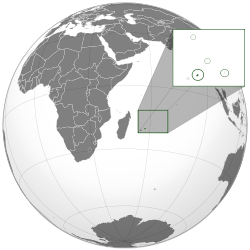
\includegraphics[width=1.0\textwidth]{images/Mauritius-Wikipedia-Position.png} 
    \end{figure}
    \end{minipage}

    \vspace{0.7cm}
    \begin{minipage}{1.0\textwidth}
    \centering
    \footnotesize
    Related work: \citep{rajah-carrim2009UseStandardisationMauritian, gobin-rahimbux2023KreolStemHybridLanguagedependent, ramsurrun2024ParsingMauritianCreole, bastien2022CaseStudyData, goodasahib-kaudeer2019AutomaticSpeechRecognition, gobin-rahimbux2023VoiceBasedPersonalAssistant, sukhoo2014TranslationEnglishMauritian, dabre2014AnouTradirExperiences, dabre2022MorisienMTDatasetMauritian}
    \end{minipage}
\end{frame}

\begin{frame}[fragile]
	\frametitle{Kurdish Kobani}
    \begin{minipage}{.70\textwidth}
    \centering
    \begin{itemize}
        \item Kurdish (Kurdî) $\rightarrow$ Kurmanji $\rightarrow$ Kobani
        \item Kurdistan has been scene of armed struggles since First World War
        \item No government that organizes or funds language research
        \item Population separated over nations and language spheres
        \item Made up of a vast dialect continuum
        \item Sorani (Central Kurdish) ~7 million Kurds
        \item Kurmanji (Northern Kurdish) ~15-20 million Kurds
        \item For a long time illegal to read and write
    \end{itemize}
    \end{minipage}%
    \begin{minipage}{.30\textwidth}
      \begin{figure}
        \centering
        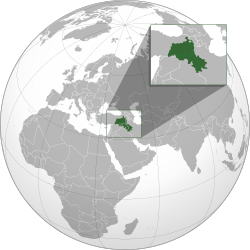
\includegraphics[width=1.0\textwidth]{images/Kurdistan-Wikipedia-Position.png} 
    \end{figure}
    \end{minipage}

    \vspace{0.7cm}
    \begin{minipage}{1.0\textwidth}
    \centering
    \footnotesize
    Related work (Kobani): \citep{ahmad2023AnalysisPhonologyMorphology, najem-aldin2021IzafeKobaniVariety} \\
    Related work (Kurmanji): \citep{morad2024PartofSpeechTaggingNorthern, gokirmak2017DependencyTreebankKurmanjia, hassani2021CanLinguisticDistance, haig2018KurmanjiKurdishTurkey, herkenrath2022MultilingualCorpusApproach, ameen2023AssessingQualityMachine, gupta2022ProgressMultilingualSpeech, thackston2006KurmanjiKurdishReference}
    \end{minipage}
\end{frame}

\begin{frame}[fragile]
	\frametitle{Vietnamese}
    \begin{minipage}{.70\textwidth}
    \centering
    \begin{itemize}
        \item Vietnamese %(Tiếng Việt)
        \item Prior to the alphabet reform, Vietnam used Chinese characters %(Chữ Nôm)
        \item When Vietnam was colonized by the French, the Latin alphabet% (Chữ Quốc Ngữ) 
        systematically replaced the Chinese characters as the written language for everybody, which greatly increased literacy in Vietnam
        \item More than 80 million native speakers
        \item Various dialects, generally mutually intelligible
        \item Vocabulary influenced by Chinese and French
    \end{itemize}
    \end{minipage}%
    \begin{minipage}{.30\textwidth}
      \begin{figure}
        \centering
        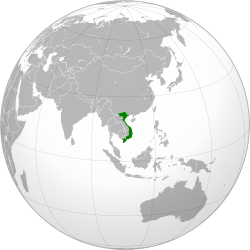
\includegraphics[width=1.0\textwidth]{images/Vietnam-Wikipedia-Position.png} 
    \end{figure}
    \end{minipage}

    \vspace{0.6cm}
    \begin{minipage}{1.0\textwidth}
    \centering
    \footnotesize
    Related work: \citep{tran2022MethodChineseVietnameseBilingual, le2023ParallelCorpusVietnamese, li2020RevisitingBackTranslationLowResource, vu2020KoreanVietnameseNeuralMachine, doan2021PhoMTHighQualityLargeScale}
    \end{minipage}
\end{frame}

\begin{frame}[fragile]
	\frametitle{Chinese}
    \begin{minipage}{.70\textwidth}
    \centering
    \begin{itemize}
        \item Chinese (simplified) 
        \begin{CJK*}{UTF8}{gbsn}(汉语)\clearpage\end{CJK*}
        \item Country in East Asia exceeding 1.4 billion inhabitants
        \item Chinese is classified into more than 10 dialect groups
        \item Many of which are mutually unintelligible
        \item A standardized writing system used for all variants
        \item Many low-resource variants, not even properly classified
        \item Standard Chinese though, provides lots of resources \& tools
        \item Proposed as alternative to English-centric NLP research
    \end{itemize}
    \end{minipage}%
    \begin{minipage}{.30\textwidth}
      \begin{figure}
        \centering
        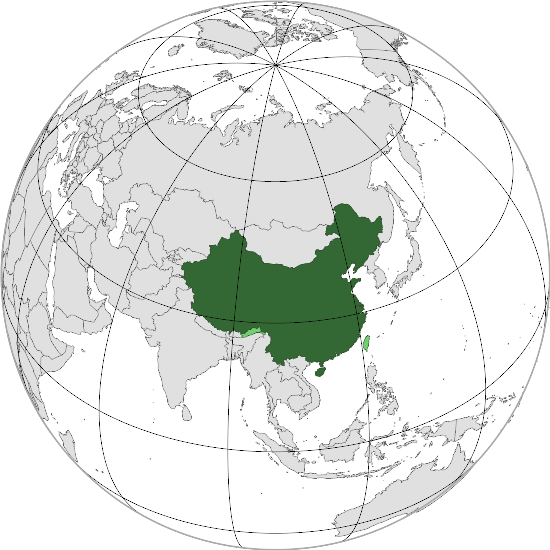
\includegraphics[width=1.0\textwidth]{images/China-Wikipedia-Position.png} 
    \end{figure}
    \end{minipage}

    \vspace{0.6cm}
    \begin{minipage}{1.0\textwidth}
    \centering
    \footnotesize
    Related work: \citep{chen2022ApproachingNeuralChinese, lei2021LeveragingZipfsLaw, xie2023CCMBLargescaleChinese, zhang2013ForcedAlignmentApproach, li2024BetterChinesecentricNeural, zhang2024NeuralMachineTranslation, dadparvar2024OrientalWhispersUnveiling}
    \end{minipage}
\end{frame}

\begin{frame}[fragile]
	\frametitle{Language Data waiting to be collected}
    \begin{figure}
	    \centering
	    \includegraphics[width=0.33\textwidth]{images/Kurmanjî-wordcloud.png}%
        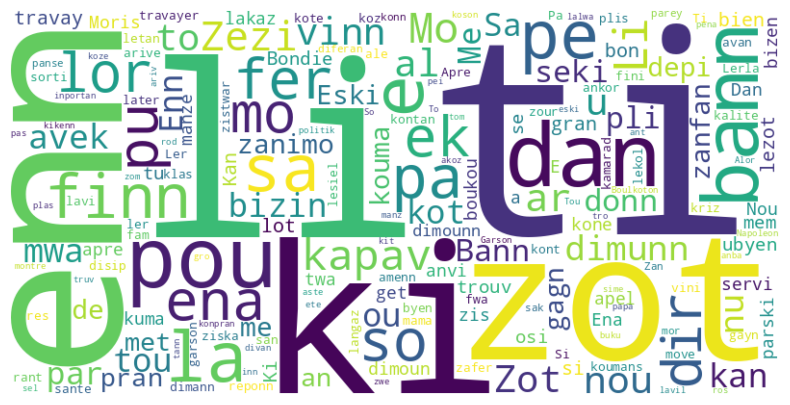
\includegraphics[width=0.33\textwidth]{images/Morisien-wordcloud.png}%
        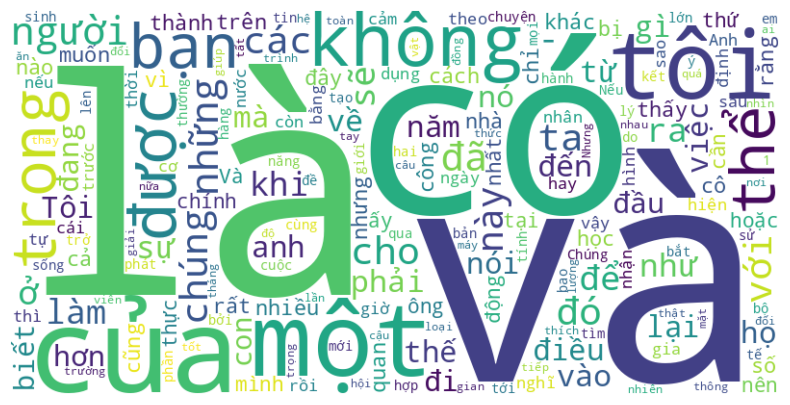
\includegraphics[width=0.33\textwidth]{images/Vietnamese-wordcloud.png}
        \\
        \includegraphics[width=0.33\textwidth]{images/Chinese-wordcloud.png}%
        \includegraphics[width=0.33\textwidth]{images/German-wordcloud.png}%
        \includegraphics[width=0.33\textwidth]{images/English-wordcloud.png}
	\end{figure}
\end{frame}


\section{Methods\&Data Quality}

\begin{frame}[fragile]
	\frametitle{Collecting Text Data}
    \begin{figure}
	    \centering
	    \includegraphics[width=.8\textwidth]{images/CRAMT-Tool-CollectWebdata.png}
	\end{figure}
\end{frame}

\begin{frame}[fragile]
	\frametitle{Bridging the Language Gap}
    \begin{figure}
	    \centering
	    \includegraphics[width=1.0\textwidth]{images/CRAMT-Tool-TextAlignmentsOverviewMulti.png}
	\end{figure}
\end{frame}

\begin{frame}[fragile]
	\frametitle{Use of Pivot Languages}
    \begin{figure}
	    \centering
	    \includegraphics[width=1.0\textwidth]{images/CRAMT-Tool-TextAlignments.png}
	\end{figure}
\end{frame}

\begin{frame}[fragile]
	\frametitle{Where to Begin?}
    \begin{minipage}{.50\textwidth}
    \centering
    Translations from English \\
    (Bilingual experts)
    \begin{figure}
        \includegraphics[width=0.2\textwidth]{images/nllb-logo.png} 
    \end{figure}
    \footnotesize 
    No Language Left Behind (NLLB) open-sources models that aim to deliver evaluated, high-quality translations directly between 200 languages. \\
    The NLLB-Seed data spans 39 languages, such as Acehnese, Bambara, Dzongkha, Friulian, Limburgish, Maori, Silesian, Venetian. \\
    \normalsize
    \textbf{6193 English sentences in NLLB-Seed.}
    \end{minipage}%
    \begin{minipage}{.50\textwidth}
    \centering
    Descriptions of Images \\
    (Monolingual native speaker)
    \begin{figure}
        \includegraphics[width=0.2\textwidth]{images/flickr30k-logo.png} 
    \end{figure}
    \footnotesize 
    The Flickr30k dataset contains images collected from Flickr, together with 5 reference sentences provided by human annotators. \\
    Has already been extended to German, French, Dutch, Chinese, Czech, Japanese, Turkish, Ukrainian, and Brazilian Portuguese.
    \normalsize
    \textbf{Approximately 31,000 images.}
    \end{minipage}
\end{frame}

\begin{frame}[fragile]
	\frametitle{Potato Annotation Tasks}
    \begin{minipage}{.10\textwidth}
        \centering
        \begin{figure}
            \includegraphics[width=1.0\textwidth]{images/mtacr-potato-login.png} 
        \end{figure}
    \end{minipage}\hfill%
    \begin{minipage}{.45\textwidth}
        \centering
        \begin{figure}
            \includegraphics[width=1.0\textwidth]{images/mtacr-potato-nllb-mfe.png} 
        \end{figure}
    \end{minipage}\hfill%
    \begin{minipage}{.35\textwidth}
        \centering
        \begin{figure}
            \includegraphics[width=1.0\textwidth]{images/mtacr-potato-flickr30k-vie.png} 
        \end{figure}
    \end{minipage}
\end{frame}

\begin{frame}[fragile]
	\frametitle{Anchor Items}
    \begin{figure}
	    \centering
	    \includegraphics[width=.70\textwidth]{images/CRAMT-Tool-AnnotationQuality.png}
	\end{figure}
\end{frame}

\section{Challenges\&Surprises}

\begin{frame}[fragile]
	\frametitle{The Usual Suspects}
    \begin{itemize}
        \item Lack of basic NLP-tools
        \item Juggling multiple writing systems
        \item Rare translators and annotators
        \item Many file formats for text corpora
        \item Minimum wage across continents
    \end{itemize}
\end{frame}


\begin{frame}[fragile]
	\frametitle{Issue with Funding? Or Issue with Bureaucracy?}
    \begin{minipage}{.45\textwidth}
        \centering
        \begin{itemize}
            \item \textbf{Regarding Translators}
            \begin{itemize}
                \item Contracts: UHH students only!
                \item Okay, non-students too...
                \item Okay, even Germany-wide...
                \item Okay, Fiverr is allowed- \\ but we don't pay, only reimburse!
            \end{itemize}
            \item \textbf{Regarding Annotators}
            \begin{itemize}
                \item Only option: Amazon.com voucher
            \end{itemize}
        \end{itemize}
    \end{minipage}%
    \begin{minipage}{.55\textwidth}
    \centering
        \begin{figure}
            \includegraphics[width=1.0\textwidth]{images/MTACR-Overview.png} 
        \end{figure}
    \end{minipage}
\end{frame}

\begin{frame}[fragile]
	\frametitle{The Story of the Unloved TXT-Template}
    \centering
    \large
    \begin{itemize}
        \item Step 1.: Send indexed files to translators
        \begin{itemize}
            \item T01-mfe.txt
            \item T03-vie.txt
            \item T07-kob.txt
        \end{itemize}
        \item Step 2.: ?
        \item Step 3.: Receive files such as
        \begin{itemize}
            \item T01-small\_01.txt\_mfe.pdf
            \item T03-vie-entire part 1-(TRANSUpdate).txt
            \item T07-kob-TRANS(3k).docx
        \end{itemize}
    \end{itemize}
\end{frame}

\begin{frame}[fragile]
	\frametitle{Fun with Experts I - (Technological) Expertise}
    \centering
    \begin{minipage}{.40\textwidth}
        \centering
        \begin{figure}
            \includegraphics[width=1.0\textwidth]{images/MTACR_fun_with_experts_001.png} 
        \end{figure}
    \end{minipage}%
    \begin{minipage}{.40\textwidth}
        \centering
        \begin{figure}
            \includegraphics[width=1.0\textwidth]{images/MTACR_fun_with_experts_002.png} 
        \end{figure}
    \end{minipage}
    \begin{minipage}{.40\textwidth}
        \centering
        \begin{figure}
            \includegraphics[width=1.0\textwidth]{images/MTACR_fun_with_experts_003.png} 
        \end{figure}
    \end{minipage}%
    \begin{minipage}{.40\textwidth}
        \centering
        \begin{figure}
            \includegraphics[width=1.0\textwidth]{images/MTACR_fun_with_experts_005.png} 
        \end{figure}
    \end{minipage}
\end{frame}

\begin{frame}[fragile]
	\frametitle{Fun with Experts II - Missed Opportunities}
    \centering
    \begin{itemize}
        \item \textbf{3 English sources}
        \begin{itemize}
            \item "0293": "There must be something in my tone of voice, or this arrogant face—something that antagonizes everybody."
            \item "0294": "In spite of his success, Warner Bros. had no interest in raising Bogart's profile."
            \item "0295": "Bogart used these years to begin developing his film persona: a wounded, stoical, cynical, charming, vulnerable, self-mocking loner with a code of honor."
        \end{itemize}
        \item \textbf{2 Vietnamese targets}
        \includegraphics[width=\textwidth]{images/challenge-vie-1.png}
        % \begin{itemize}
        % \begin{otherlanguage*}{vietnamese}
        %     \item "0293": "Bất chấp thành công của mình, hãng Warner Bros. thể hiện ít sự quan tâm trong việc nâng cao vị thế của Bogart."
        %     \item "0294": ???
        %     \item "0295": "Bogart bắt đầu hình thành nhân vật điện ảnh của mình trong những năm này, chế tác một nhân vật bị tổn thương, khắc khổ, hoài nghi, quyến rũ, dễ bị tổn thương và tự chế giễu, nhưng duy trì một quy tắc danh dự."
        % \end{otherlanguage*}
        % \end{itemize}
    \end{itemize}
\end{frame}

\begin{frame}[fragile]
	\frametitle{Fun with Experts III - Generosity}
    \centering
    \begin{itemize}
        \item \textbf{1 English source}
        \begin{itemize}
            \item "0040": "Lloyd and Roach parted ways in 1924, and Lloyd became the independent producer of his own films."
        \end{itemize}
        \item \textbf{2 Vietnamese targets}
        \includegraphics[width=\textwidth]{images/challenge-vie-2.png}
        % \begin{itemize}
        % \begin{otherlanguage*}{vietnamese}
        %     \item "0040": "Lloyd và Roach chia tay nhau vào năm 1924. Sau đó, Lloyd trở thành nhà sản xuất độc lập cho các bộ phim của riêng mình."
        %     \item "0040": "Lloyd và Roach đường ai lối khác vào năm 1924, và Lloyd bắt đầu tự sản xuất phim."
        % \end{otherlanguage*}
        % \end{itemize}
    \end{itemize}
\end{frame}

\begin{frame}[fragile]
	\frametitle{Fun with Experts IV - Creative Writing}
    \centering
    \begin{itemize}
        \item \textbf{2 English sources}
        \begin{itemize}
            \item "0266": "Maud was a commercial illustrator who received her art training in New York and France, including study with James Abbott McNeill Whistler."
            \item "0267": "She earned over 50,000 dollar a year at the peak of her career - a very large sum of money at the time, and considerably more than her husband's 20,000."
        \end{itemize}
        \item \textbf{1 Vietnamese target}
        \includegraphics[width=\textwidth]{images/challenge-vie-3.png}
        
        % \begin{itemize}
        %     \item "0266": "Maud là một họa sĩ minh họa thương mại thành công, kiếm được hơn 50,000 đô la hàng năm vào thời kỳ đỉnh cao, một khoản tiền đáng kể so với thu nhập 20,000 đô la của chồng bà."
        % \end{itemize}
    \end{itemize}
\end{frame}

\begin{frame}[fragile]
	\frametitle{Fun with Experts V - Additional Value}
    \centering
    \begin{itemize}
        \item \textbf{1 English source}
        \begin{itemize}
            \item "0064": "But they taught themselves to reason."
        \end{itemize}
        \item \textbf{1-3 Morisien targets (?)}
        \begin{itemize}
            \item "0064": "Me zot ti aprann zotmem rezone/reflesi/panse."
            \item $\rightarrow$ "Me zot ti aprann zotmem rezone."
            \item $\rightarrow$ "Me zot ti aprann zotmem reflesi."
            \item $\rightarrow$ "Me zot ti aprann zotmem panse."
        \end{itemize}
    \end{itemize}
\end{frame}

\section{Corpus Data\&Evaluation}

\begin{frame}[fragile]
	\frametitle{Collected Data}
    \centering
    \hfill\begin{figure}
        \begin{overprint}
        \centering
            \onslide<1> \includegraphics[height=6.6cm]{images/mtacr-2024-april.png} 
            \onslide<2> \includegraphics[height=6.6cm]{images/mtacr-2024-april-targets.png} 
            \onslide<3> \includegraphics[height=6.6cm]{images/mtacr-2024-april-noeng.png}  
            \onslide<4> \includegraphics[height=6.6cm]{images/mtacr-2024-april-all.png} 
        \end{overprint}
        
    \end{figure}
\end{frame}

% \begin{frame}[fragile]
% 	\frametitle{Collected Data I}
%     \begin{figure}
%     \centering
%         \includegraphics[width=1.0\textwidth]{images/mtacr-2024-april.png} 
%     \end{figure}
% \end{frame}

% \begin{frame}[fragile]
% 	\frametitle{Collected Data II}
%     \begin{figure}
%     \centering
%         \includegraphics[width=1.0\textwidth]{images/mtacr-2024-april-targets.png} 
%     \end{figure}
% \end{frame}

% \begin{frame}[fragile]
% 	\frametitle{Collected Data III}
%     \begin{figure}
%     \centering
%         \includegraphics[width=1.0\textwidth]{images/mtacr-2024-april-noeng.png} 
%     \end{figure}
% \end{frame}

% \begin{frame}[fragile]
% 	\frametitle{Collected Data IV}
%     \begin{figure}
%     \centering
%         \includegraphics[width=1.0\textwidth]{images/mtacr-2024-april-all.png} 
%     \end{figure}
% \end{frame}

\begin{frame}[fragile]
	\frametitle{Corpus Statistics (Flickr30k-based Data)}
    \begin{figure}
    \centering
        \includegraphics[width=1.0\textwidth]{images/MTACR-Corpus_statistics_for_Flickr30k_dataset.png} 
    \end{figure}
\end{frame}

\begin{frame}[fragile]
	\frametitle{Corpus Statistics (NLLB-based Data)}
    \begin{figure}
    \centering
        \includegraphics[height=6.5cm]{images/MTACR-Corpus_statistics_for_NLLB_dataset.png} 
    \end{figure}
\end{frame}

\begin{frame}[fragile]
	\frametitle{Corpus Statistics (NLLB-based Data - MT in Detail)}
    \begin{figure}
    \centering
        \includegraphics[width=1.0\textwidth]{images/MTACR-Total_sentences_for_each_translation_system_and_language.png} 
    \end{figure}
\end{frame}

\begin{frame}[fragile]
	\frametitle{MT Versus Humans I - BLEU}
    \begin{minipage}{.33\textwidth}
    \begin{figure}
        \centering
        \includegraphics[width=1.0\textwidth]{images/eval-01-Chinese-Anchors-bleu.png} 
    \end{figure}
    \end{minipage}%
    \begin{minipage}{.33\textwidth}
    \begin{figure}
        \centering
        \includegraphics[width=1.0\textwidth]{images/eval-01-Vietnamese-Anchors-bleu.png} 
    \end{figure}
    \end{minipage}%
        \begin{minipage}{.33\textwidth}
    \begin{figure}
        \centering
        \includegraphics[width=1.0\textwidth]{images/eval-01-Morisien-Anchors-bleu.png} 
    \end{figure}
    \end{minipage}
\end{frame}

\begin{frame}[fragile]
	\frametitle{MT Versus Humans II - Chinese}
    \begin{minipage}{1.0\textwidth}
    \begin{figure}
        \centering
        \includegraphics[width=1.0\textwidth]{images/eval-01-Chinese-Anchors.png} 
    \end{figure}
    \end{minipage}
\end{frame}

\begin{frame}[fragile]
	\frametitle{MT Versus Humans III - Vietnamese}
    \begin{minipage}{1.0\textwidth}
    \begin{figure}
        \centering
        \includegraphics[width=1.0\textwidth]{images/eval-01-Vietnamese-Anchors.png} 
    \end{figure}
    \end{minipage}
\end{frame}

\begin{frame}[fragile]
	\frametitle{MT Versus Humans IV - Morisien}
    \begin{minipage}{1.0\textwidth}
    \begin{figure}
        \centering
        \includegraphics[width=1.0\textwidth]{images/eval-01-Morisien-Anchors.png} 
    \end{figure}
    \end{minipage}
\end{frame}

\begin{frame}[fragile]
	\frametitle{Cross-lingual Aligned Words}
    \begin{figure}
        \centering
        \includegraphics[width=0.8\textwidth]{images/TextAsCorpusRep-Concept-TextAlignmentsOverviewTable.png} 
    \end{figure}
\end{frame}

\section{Next Steps}


\begin{frame}[fragile]
	\frametitle{Bilingual Lexicon Induction}
    \begin{figure}
        \centering
        \includegraphics[width=0.8\textwidth]{images/ChameleonMT-BLI-BLI.png}
        \caption{Inspiration for this figure: (Wang et al., 2021) and (Irvine and Callison-Burch, 2017).}
    \end{figure}
\end{frame}


\begin{frame}[fragile]
	\frametitle{Dialect Filters - Dialect (Multi-)Labels}
    \begin{minipage}{.50\textwidth}
    \begin{figure}
        \centering
        \includegraphics[width=1.0\textwidth]{images/DialectFilters-Overview.png} 
    \end{figure}
    \end{minipage}%
    \begin{minipage}{.50\textwidth}
    \begin{figure}
        \centering
        \includegraphics[width=1.0\textwidth]{images/DialectFilters-PipelineOverview.png} 
    \end{figure}
    \end{minipage}
\end{frame}



\begin{frame}[fragile]
	\frametitle{MTACR's Future (Short-Term) - Improve \& Enhance I}
    \begin{minipage}{.50\textwidth}
    \footnotesize
    \textbf{Human Study \& Data Selection}
    \begin{itemize}
        \item Human evaluation to leave BLEU behind
        \item TrueSkill for higher information gain \citep{herbrich2006TrueSkillBayesianSkill, minka2018TrueSkill2Improveda}
        \item Cross-lingual sentence representations \citep{kowtal2024DataSelectionApproach} % (Kowtal et al., 2024)
        \item Active learning and Self-training \citep{schroder2024SelfTrainingSampleEfficientActive} % (Schröder and Heyer, 2024)
    \end{itemize}
    \textbf{Structured Data}
    \begin{itemize}
        \item ConceptNet \citep{speer2018ConceptNet55Open}
        \item Language-specific WordNet \citep{aliabadi2014BuildingKurdNetKurdish}
    \end{itemize}
    \end{minipage}%
    \begin{minipage}{.50\textwidth}
    \footnotesize
    \textbf{Data Post-Processing}
    \begin{itemize}
        \item Iron out the last alignment-flaws
        \item Parsing morphological rich languages \citep{tsarfaty2013ParsingMorphologicallyRich} %(Tsarfaty et al., 2013)
        \item Script normalization \citep{ahmadi2023ScriptNormalizationUnconventional, ahmadi2023PALILanguageIdentification}
        \item Improve POS-taggins \citep{morad2024PartofSpeechTaggingNorthern}
    \end{itemize}
    \textbf{Utilize Monolingual Data}
    \begin{itemize}
        \item For low-resource MT \citep{karakanta2018NeuralMachineTranslation} %(Karakanta et al., 2018)
        \item Revisit CommonCrawl \citep{kargaran2024GlotCCOpenBroadCoverage}, Opus \citep{tiedemann2012ParallelDataTools}, ... 
    \end{itemize}
    \end{minipage}
\end{frame}

\begin{frame}[fragile]
	\frametitle{MTACR's Future (Short-Term) - Improve \& Enhance II}
    \begin{minipage}{.50\textwidth}
    \footnotesize
    \textbf{Text Resources}
    \begin{itemize}
        \item Create stopword lists
        \item Universal Dependencies tag \citep{demarneffe2021UniversalDependencies}
        \item CoNLL-U format \citep{buchholz2006CoNLLXSharedTask}
        \item GrEmLIn \citep{gurgurov2025GrEmLInRepositoryGreen} % (Gurgurov et al., 2025a)
        \item GloVe \citep{pennington2014GloVeGlobalVectors}
    \end{itemize}
    \textbf{Merging Corpora}
    \begin{itemize}
        \item Multi-label classification \citep{bernier-colborne2023DialectVariantIdentification, marchal2022EstablishingAnnotationQuality, fornaciari2021BlackWhiteLeveraging, plank2022ProblemHumanLabel}
        \item Inflections \citep{metheniti2020WikinflectionCorpusBetter} % (Metheniti and Neumann, 2020)
        \item Kurdish varieties \citep{ahmadi2023ApproachesCorpusCreation, ahmadi2022LeveragingMultilingualNews}
        \item Dialect varieties \citep{alam2023CODETBenchmarkContrastive}
    \end{itemize}
    \end{minipage}%
    \begin{minipage}{.50\textwidth}
    \footnotesize
    \textbf{Cross-lingual Alignment}
    \begin{itemize}
        \item Morphological rich \citep{ustun2019CrossLingualWordEmbeddingsMorphologically} % (Üstün et al., 2019)
        \item Text alignment \citep{artetxe2019MassivelyMultilingualSentence} % (Artetxe and Schwenk, 2019)
        \item BLI \citep{bafna2024WhenYourCousin, bafna2023SimpleMethodUnsupervised, artemova2023LowresourceBilingualDialect}
        \item In-context word alignments \citep{martelli2023XLWAGoldEvaluation} % (Martelli et al., 2023)
    \end{itemize}
    \textbf{Translation Directions}
    \begin{itemize}
        \item Explore Backtranslation \citep{edunov2018UnderstandingBackTranslationScale}
        \item Multi-Pivot Ensembling \citep{mohammadshahi2023InvestigatingMultiPivotEnsembling} % (Mohammadshahi et al., 2023)
    \end{itemize}
    \end{minipage}
\end{frame}

\begin{frame}[fragile]
	\frametitle{MTACR's Future (Long-Term) - Explore \& Investigate}
    \begin{minipage}{.50\textwidth}
    \footnotesize
    \textbf{LLMs for Low-resource MT}
    \begin{itemize}
        \item Claude \citep{enis2024LLMNMTAdvancing} % (Enis and Hopkins, 2024)
        \item General \citep{richburg2024HowMultilingualAre} % (Richburg and Carpuat, 2024)
        \item Different application domains \citep{zheng2024HowWellLLMs} % (Zheng et al., 2024)
        \item Prompting strategies \citep{schulhoff2024PromptReportSystematic} % (Schulhoff et al., 2024)
        \item Soft prompting \citep{vykopal2024SoftLanguagePrompts} % (Vykopal et al., 2024)
        \item Unsupervised data generation for self-supervised NMT \citep{ruiter2021IntegratingUnsupervisedDataa} % (Ruiter et al., 2021)
        \item Explore model fine-tuning
    \end{itemize}
    \end{minipage}%
    \begin{minipage}{.50\textwidth}
    \footnotesize
    \textbf{Adapting}
    \begin{itemize}
        \item Language adapters \citep{gurgurov2024AdaptingMultilingualLLMs, parovic2022BADXBilingualAdapters, ustun2022UDapterTypologybasedLanguage} % (Gurgurov et al., 2024) (Parović et al., 2022) (Üstün et al., 2022)
        \item Task adapters \citep{held2023TADATaskAgnosticDialect, pfeiffer2021AdapterFusionNonDestructiveTask, pfeiffer2020MADXAdapterBasedFramework} % (Held et al., 2023) (Pfeiffer et al., 2021, 2020)
        \item Vocabulary altering adapters \citep{han2024AdaptersAlteringLLM} % (Han et al., 2024)
    \end{itemize}
    \textbf{Going Small}
    \begin{itemize}
        \item Minimal data \citep{maillard2023SmallDataBig} % (Maillard et al., 2023)
        \item Small models \citep{gurgurov2025SmallModelsBig} % (Gurgurov et al., 2025b)
        \item Smalles comprehensive model \citep{eldan2023TinyStoriesHowSmall} % (Eldan 2023) 
    \end{itemize}
    \end{minipage}
\end{frame}



\begin{frame}[fragile]
	\frametitle{La Ende}
    \Large Questions now, cake later? 
\end{frame}


%\section{References}
\begin{frame}[allowframebreaks, fragile]
	\frametitle{References}
	% \bibliographystyle{alpha}
    \bibliographystyle{apalike}
    %\bibliographystyle{authoryear}
    \tiny
	\bibliography{BetterBibTex}
    %\nocite{*}
    %\bibliography{literature}
\end{frame}




\section{Appendix}


\begin{frame}[fragile]
	\frametitle{Example I: Flickr30k-0001}
    \begin{minipage}{.50\textwidth}
    \begin{figure}
        \centering
        \includegraphics[width=1.0\textwidth]{images/13651137.jpg} 
    \end{figure}
    \end{minipage}%
    \begin{minipage}{.50\textwidth}
    \includegraphics[width=\textwidth]{images/example-flikr-1.png}
    % \textbf{Kobani}
    % \begin{itemize}
    %     \item "mêrkek bi kombrêsê erdê xerab dikê"
    % \end{itemize}
    % \textbf{Morisien}
    % \begin{itemize}
    %     \item "enn missier p craze simin avec so machine craz roche"
    % \end{itemize}
    % \textbf{Vietnamese}
    % \begin{itemize}
    %     \item "Một công nhân xây dựng đang làm việc với một búa khoan."
    %     \item "Anh ấy đang phá dỡ đường"
    % \end{itemize}
    % \textbf{Chinese}
    % \begin{itemize}
    %     \begin{CJK*}{UTF8}{gbsn}
    %     \item "一名工人正在拆除房屋前面的水泥路面"
    %     \clearpage\end{CJK*}
    % \end{itemize}
    \end{minipage}
\end{frame}

\begin{frame}[fragile]
	\frametitle{Example II: NLLB-0001}
    \includegraphics[width=\textwidth]{images/example-nllb-1.png}
    % \textbf{English}
    % \begin{itemize}
    %     \item "Lillian Diana Gish (October 14, 1893 – February 27, 1993) was an American actress, director and screenwriter."
    % \end{itemize}
    % \textbf{Morisien}
    % \begin{itemize}
    %     \item "Lillian Diana Gish (inn ne 14 Oktob 1893 – inn mor 27 Fevrie 1993) li ti enn akter, enn realizater ek enn senaris Amerikenn."
    %     \item "Lillian Diana Gish (14 Oktob 1893 - 27 Fevriye 1993) ti enn aktris, realizatris ek senarist amerikenn."
    % \end{itemize}
    % \textbf{Vietnamese}
    % \begin{itemize}
    %     \item "Lillian Diana Gish, sinh ngày 14 tháng 10 năm 1893 và mất ngày 27 tháng 2 năm 1993, là một nữ diễn viên, đạo diễn và biên kịch người Mỹ."
    %     \item "Lillian Diana Gish (14/10/1893 – 27/2/1993) là một nữ diễn viên, đạo diễn, biên kịch người Mỹ."
    %     \item "Lillian Diana Gish (14/10/1893 – 27/02/1993) là một nữ diễn viên, đạo diễn và nhà biên kịch người Mỹ."
    % \end{itemize}
    % \textbf{Kobani}
    % \begin{itemize}
    %     \item "Lillian Diana Gish (14'î mehê 10'an 1893 - 27'î mehê didîyan 1993) lîstikvan, derhêner û sînaronivîseke Emrîkî bû."
    %     \item "Lilian Diana Gish (14î meha dehan, 1893 - 27î meha didiyan , 1993) lîstikvan, derhêner, û senarîsteke Emrîkî bû."
    % \end{itemize}
    % \textbf{Chinese}
    % \begin{itemize}
    %     \begin{CJK*}{UTF8}{gbsn}
    %     \item "莉莲·戴安娜·吉什(1893年10月14日-1993年2月27日),美国女演员、导演和编剧。"
    %     \item "莉莲·戴安娜·吉什(1893年10月14日-1993年2月27日)是一位美国女演员、导演和编剧。"
    %     \item "莉莉安·黛安娜·吉许(1893年十月十四日-1993年二月27日)是一个美国演员,导演和编剧。"
    %     \clearpage\end{CJK*}
    % \end{itemize}
\end{frame}



\begin{frame}[fragile]
	\frametitle{Language Ambiguity}
    \begin{figure}
        \centering
        \includegraphics[width=1.0\textwidth]{images/CRAMT-Tool-WordAlignmentExample.png} 
    \end{figure}
\end{frame}

\begin{frame}[fragile]
	\frametitle{Language Ambiguity a Limitation?}
    \begin{figure}
        \centering
        \includegraphics[width=1.0\textwidth]{images/CRAMT-Tool-WordAlignmentLimitation.png} 
    \end{figure}
\end{frame}

\begin{frame}[fragile]
	\frametitle{Language Ambiguity a Potential?}
    \begin{figure}
        \centering
        \includegraphics[width=1.0\textwidth]{images/CRAMT-Tool-WordAlignmentLimitationExample.png} 
    \end{figure}
\end{frame}


\begin{frame}[fragile]
	\frametitle{MT Evaluation - BLEU}
    \begin{figure}
        \centering
        \includegraphics[width=0.75\textwidth]{images/ChameleonMT-EVAL-BLEU.png}
    \end{figure}
\end{frame}

\begin{frame}[fragile]
	\frametitle{MT Evaluation - chrF}
    \begin{figure}
        \centering
        \includegraphics[width=0.87\textwidth]{images/ChameleonMT-EVAL-chrF.png}
    \end{figure}
\end{frame}

\begin{frame}[fragile]
	\frametitle{MT Evaluation - TER}
    \begin{figure}
        \centering
        \includegraphics[width=1.0\textwidth]{images/ChameleonMT-EVAL-TER.png}
    \end{figure}
\end{frame}


\end{document}
